\chapter{Peirce's Notes on Triadic Logic}

%It is no secret that Peirce never reached the level of success that would have allowed him to publish as voluminously as he wrote within his lifetime.

%As such, 
Peirce's mature philosophy, along with his work on logic and set theory, is contained within a collection of unpublished manuscripts. One of these manuscripts, simply entitled ``The Logic Notebook,'' was a notebook where Peirce first set out and tested his ideas. Peirce wrote in this notebook periodically for most of his life. The first entry is dated November 12, 1865, while the final entry does not occur until November 1, 1909. At some point, these notes were separated and scattered amongst several files and remained  that way until the notebook was reassembled by Don Roberts in \href{https://iiif.lib.harvard.edu/manifests/view/drs:15255301$1i}{1961}. By 1964 they were reproduced on microfilm for viewing. Now images of the pages have been reproduced \href{https://iiif.lib.harvard.edu/manifests/view/drs:15255301$637i}{online}\footnote{https://iiif.lib.harvard.edu/manifests/view/drs:15255301$637i} as part of the Houghton Library's digitization initiative at Harvard. It is in this notebook that we find the three pages that have garnered Peirce attention for being an early pioneer of many-valued logic.

The first two pages where the use of a third truth value appear are both undated \textit{versos}. They were likely written between January 7th, 1909, and February 17th, 1909, judging by the dates on the other surrounding pages. The \textit{recto} between the two \textit{versos} is dated February 16th, and the one following the second page is dated the 17th. Of the pages Fisch and Turquette draw attention to, the only one that has been dated is  February 23rd, 1909. Fisch and Turquette were the first to notice and publish these pages in \citeyear{fisch_peirces_1966}.

All of the research on Peirce's triadic logic so far has focused on these three pages, however further examination of the surrounding pages reveals some obvious connections between triadic logic and other topics Peirce was working out at the time. The reason that most scholarship has neglected the other relevant pages is unclear. It is likely due to the fact that those were the only pages Fisch and Turquette decided to focus on when they wrote the first paper on the subject \citep{fisch_peirces_1966}. Since access to the original manuscript pages was limited until recently, their decision is likely the reason other scholars do not seem to have noticed these other pages. As ``The Logic Notebook'' had already been reassembled by the time Fisch and Turquette were writing, it is unlikely that they would not have seen the additional pages, which makes their decision not to mention them puzzling. 

The present chapter is devoted to providing an accurate description of the relevant pages from ``The Logic Notebook.'' I will first take up the three pages that have received the most discussion from other researchers on the subject. I will then discuss the additional pages that have hitherto been omitted. Throughout the section I will sometimes use numbers in parenthesis to indicate the parts on the page under current discussion. These numbers correspond to the numbers on the annotated images of the pages given as figures in their respective sections. The order in which the pages are discussed is not exactly the order they were chronologically written. I give priority to the pages that have already been taken up by others before examining those that have not. The order they likely would have been arranged when the notebook was in its original condition can be determined by reference to their seq. numbers. The first page related to Peirce's triadic logic is \href{https://iiif.lib.harvard.edu/manifests/view/drs:15255301$637i}{seq. 637} and the last is \href{https://iiif.lib.harvard.edu/manifests/view/drs:15255301$645i}{seq. 645}. It is possible that the undated \textit{versos} could have been afterthoughts, written after Peirce had come back and reflected upon the dated pages. There is one page that falls within the range between seq. 637--645 that I have not included in this discussion. That is \href{https://iiif.lib.harvard.edu/manifests/view/drs:15255301$643i}{seq. 643}, which is entitled ``Geometrical Topics."\footnote{This page was excluded because it did not initially appear to be relevant to Peirce's triadic logic. However, as Peirce's intentions become clearer, in light of this thesis, it might turn out to be relevant after all.} In the pages leading up to the triadic logic notes, Peirce was making notes on a paper for the American Mathematical Society, that was to be called ``Logical Remarks on Some Mathematical Definitions" (\href{https://iiif.lib.harvard.edu/manifests/view/drs:15255301$631i}{seq. 631} and onward). This paper does not appear ever to have been completed or published. The page immediately following the triadic logic notes, is a ``Note on the Tinctures," which turns out to be related to another system of logic, Peirce's Tinctured Gamma Graphs (\href{https://iiif.lib.harvard.edu/manifests/view/drs:15255301$646i}{seq. 646}).\footnote{See \cite{pietarinen_peirces_2006} for discussion of Tinctured Graphs.}
%Squeeze this down, the surrounding pages give great evidence...

\section{seq. 638 V.}

\begin{figure}
    \centering
    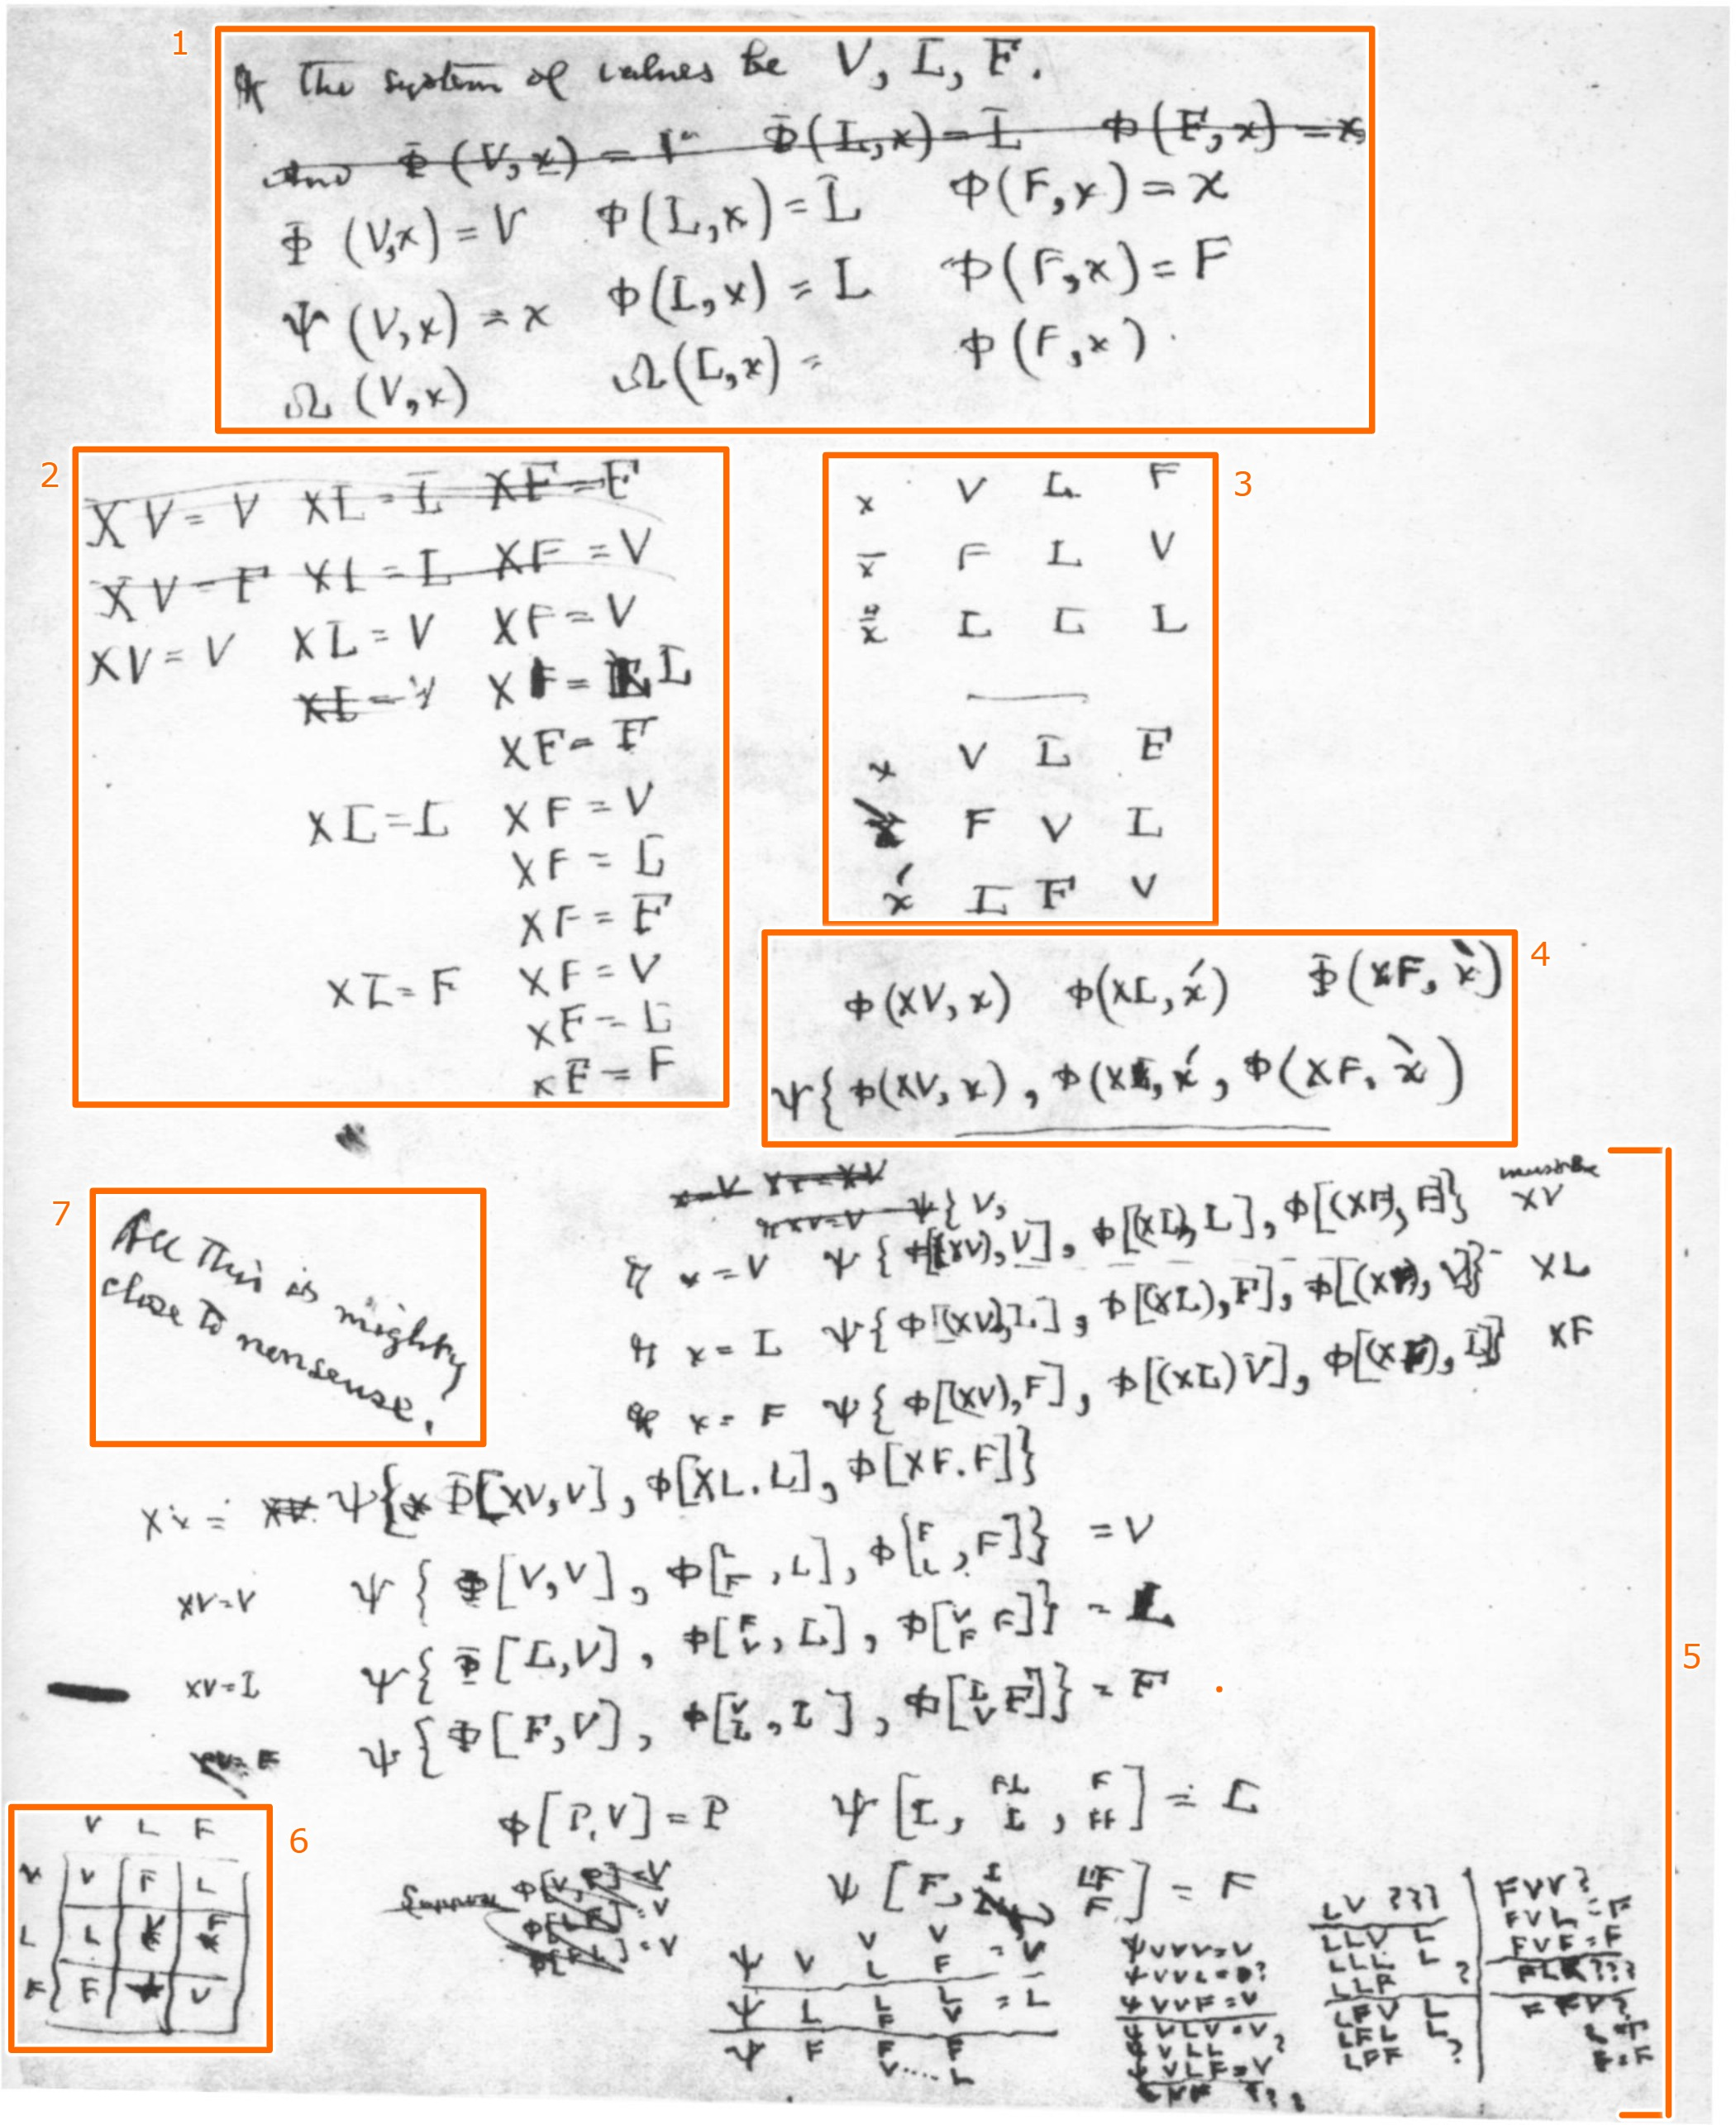
\includegraphics[width=\textwidth]{images/page one.jpeg}
    \caption{First Page, \href{https://iiif.lib.harvard.edu/manifests/view/drs:15255301$638i}{seq. 638 V.}}
    \label{fig:seq638}
\end{figure}



The first page begins (1) ``Let$[\!\![$?$]\!\!]$\footnote{There are times when Peirce's writing is illegible, reducing confidence in the accuracy of my transcriptions. In these cases I will put a `?' in double square braces to indicate the possibility of error. When these marks appear without the braces they are part of the original manuscript.} the system of values be $V, L, F$.'' The first line is crossed out and appears to have read ``And $ \Phi(V,x)=F$[\!\![$?$]\!\!]$ \enspace \Phi(L,x)=L	\enspace	\Phi(F,x)=x$.'' The first definitions are for the $\Phi$, $\Psi$, and $\Omega$ operators.
\begin{gather*}
\Phi(V, x)= V, \enspace \Phi(L,x)=L, \enspace \Phi(F, x)=x\\
\Psi(V,x)=x, \enspace \Phi(L, x)=L, \enspace \Phi(F,x)=F\\
\Omega(V,x), \quad \Omega(L,x)=\enspace, \quad \Phi(F,x)
\end{gather*}
Presumably the $x$ in these formula can take any value, so the first formula of the top line should be read as `phi of a \textit{verum} proposition and any proposition is \textit{verum}.' Peirce seems to have been focused mainly on defining the $\Phi$ operator on this page. The crossed out line conflicts with the first formula of the top line. The middle line conflicts with the top in the third formula, but it agrees with the crossed out first line in this regard. These disagreements seem to indicate a certain amount of indecision on Peirce's part and it is difficult to tell what kind of connective he wanted $\Phi$ to be. The middle line also introduces the $\Psi$ operator, but only provides one valuation for it. The third line introduces $\Omega$ but does not give any valuations for the formulae on it.

Immediately below on the left (2), there appears to be some scratch work made in an attempt to define a one place operator $X$\footnote{It is typographically difficult to make clear, but this character is meant to be the greek letter Chi.}. The valuations are sorted into three columns based on whether $X$ is operating on $V, L,$ or $F$. Peirce seems to have confidence that $XV=V$, but waffled over the value of $X$ of $L$ and $F$. In the second and third columns he has listed all the possible valuations for when $X$ is applied to $L$ or $F$. He may have just wanted to write all of the combinations down to keep track of the possibilities. Another possible interpretation is that these equations were shorthand for combinations and valuations of $\Phi$, $\Psi$, or $\Omega$ formulae. The issue with this interpretation is that on other pages (seq.639 and 641), $X$ is clearly a unary operator.

To the right (3) appears to be the only part of the first page deemed worth salvaging. Here Peirce defines four unary operators. $\bar{\lnot}x$\footnote{While Peirce uses different accents to symbolize his various negations, like $\bar{x}$, $\mathring{\bar{x}}$, $\acute{x}$, and $\grave{x}$, I have elected to use prefix operators, $\bar{\lnot}x$,  $\mathring{\bar{\lnot}}x$, $\diagdown{x}$, and $\diagup{x}$, instead.} appears to be the standard interpretation of negation in three valued logic and is common to Łukasiewicz's system. $\mathring{\bar{\lnot}}x$ is the operator that gives $L$ no matter the input. It corresponds to Slupecki's ``tertium function" \citeyearpar{slupecki_volle_1937} and could be used as a constant of sorts. (It may also be possible to define modal functors with $\mathring{\bar{\lnot}}x$.) $\diagdown{x}$ and $\diagup{x}$ match up with two negations that Post defines in his system. These negations turn out to be rather important for Turquette when he shows that Peirce's semantics are functionally complete and when he extends this system into a sound and complete logic. Out of the four unary operators on the page, only $\diagdown{x}$ and $\diagup{x}$ are what Turquette calls total negations. This is because out of the four they are the only ones that transform all of the values for whatever they are applied to. $\bar{\lnot}x$ and $\mathring{\bar{\lnot}}x$ only transform two of the values and keep $L$ the same. $\diagdown{x}$ and $\diagup{x}$ have an oddly cyclical nature. Notice that $\diagdown{}(\diagdown{}(\diagdown{x}))=x=\diagup{}(\diagup{}(\diagup{x})$. \footnote{Perhaps there is some connection with the cyclical arithmetic that Peirce discusses in his ``Amazing Mazes'' articles in \textit{The Monist} written around the same time \citep{peirce_amazing_1908}.}

\begin{displaymath}
\begin{array}{|c|c|c|c|c|}
% |c c|c| means that there are three columns in the table and
% a vertical bar ’|’ will be printed on the left and right borders,
% and between the second and the third columns.
% The letter ’c’ means the value will be centered within the column,
% letter ’l’, left-aligned, and ’r’, right-aligned.
p & \bar{\lnot}x & \diagdown{p} & \diagup{p} & \mathring{\bar{\lnot}}p\\ % Use & to separate the columns
\hline % Put a horizontal line between the table header and the rest.
V & F & F & L & L\\
L & L & V & F & L\\
F & V & L & V & L\\
\end{array}
\end{displaymath}

Immediately below the unary operators (4), Peirce appears to be experimenting with $\Phi$, $\Psi$ and the two cyclical negations. The other more mysterious unary operator, $X$, also features in these formulae. It is unclear what the point of this was.

Little can be gleaned from the area (5) immediately below either since it is not clear what $XV, XL,$ or $XF$ express unless they somehow match up with the work done in (2). This seems unlikely though because the values on any combination other than $XV$ in (2) are ill defined. He seems to have been trying to work out $\Psi$ however, here it appears as a three place operator. Its being considered as a three place operator is demonstrated by the array on the bottom right of the page and by its taking of three $\Phi$ formulae as arguments above this. However, these would still make sense if $\Psi$ was a two place operator, as long as it was associative.

On the bottom left of the page (6) there is a characteristic matrix for some undisclosed operator. It does not to match up with any of the completed matrices that appear on the next page under discussion, seq. 640.

In the middle of the left (7) we find what is perhaps Peirce's admission of defeat. The text reads ``all this is mighty close to nonsense." It seems he was ultimately unsatisfied with the work done on this page. His primary concern here seems to be working out definitions for $\Phi$ and $\Psi$ and possibly some relationship between the two, as shown by the nesting of $\Phi$ formulae within $\Psi$ formulae. Since the Post negations also feature in some of these formulae, its possible that they played a role in this relationship.

\section{seq. 640 V.}

\begin{figure}
    \centering
    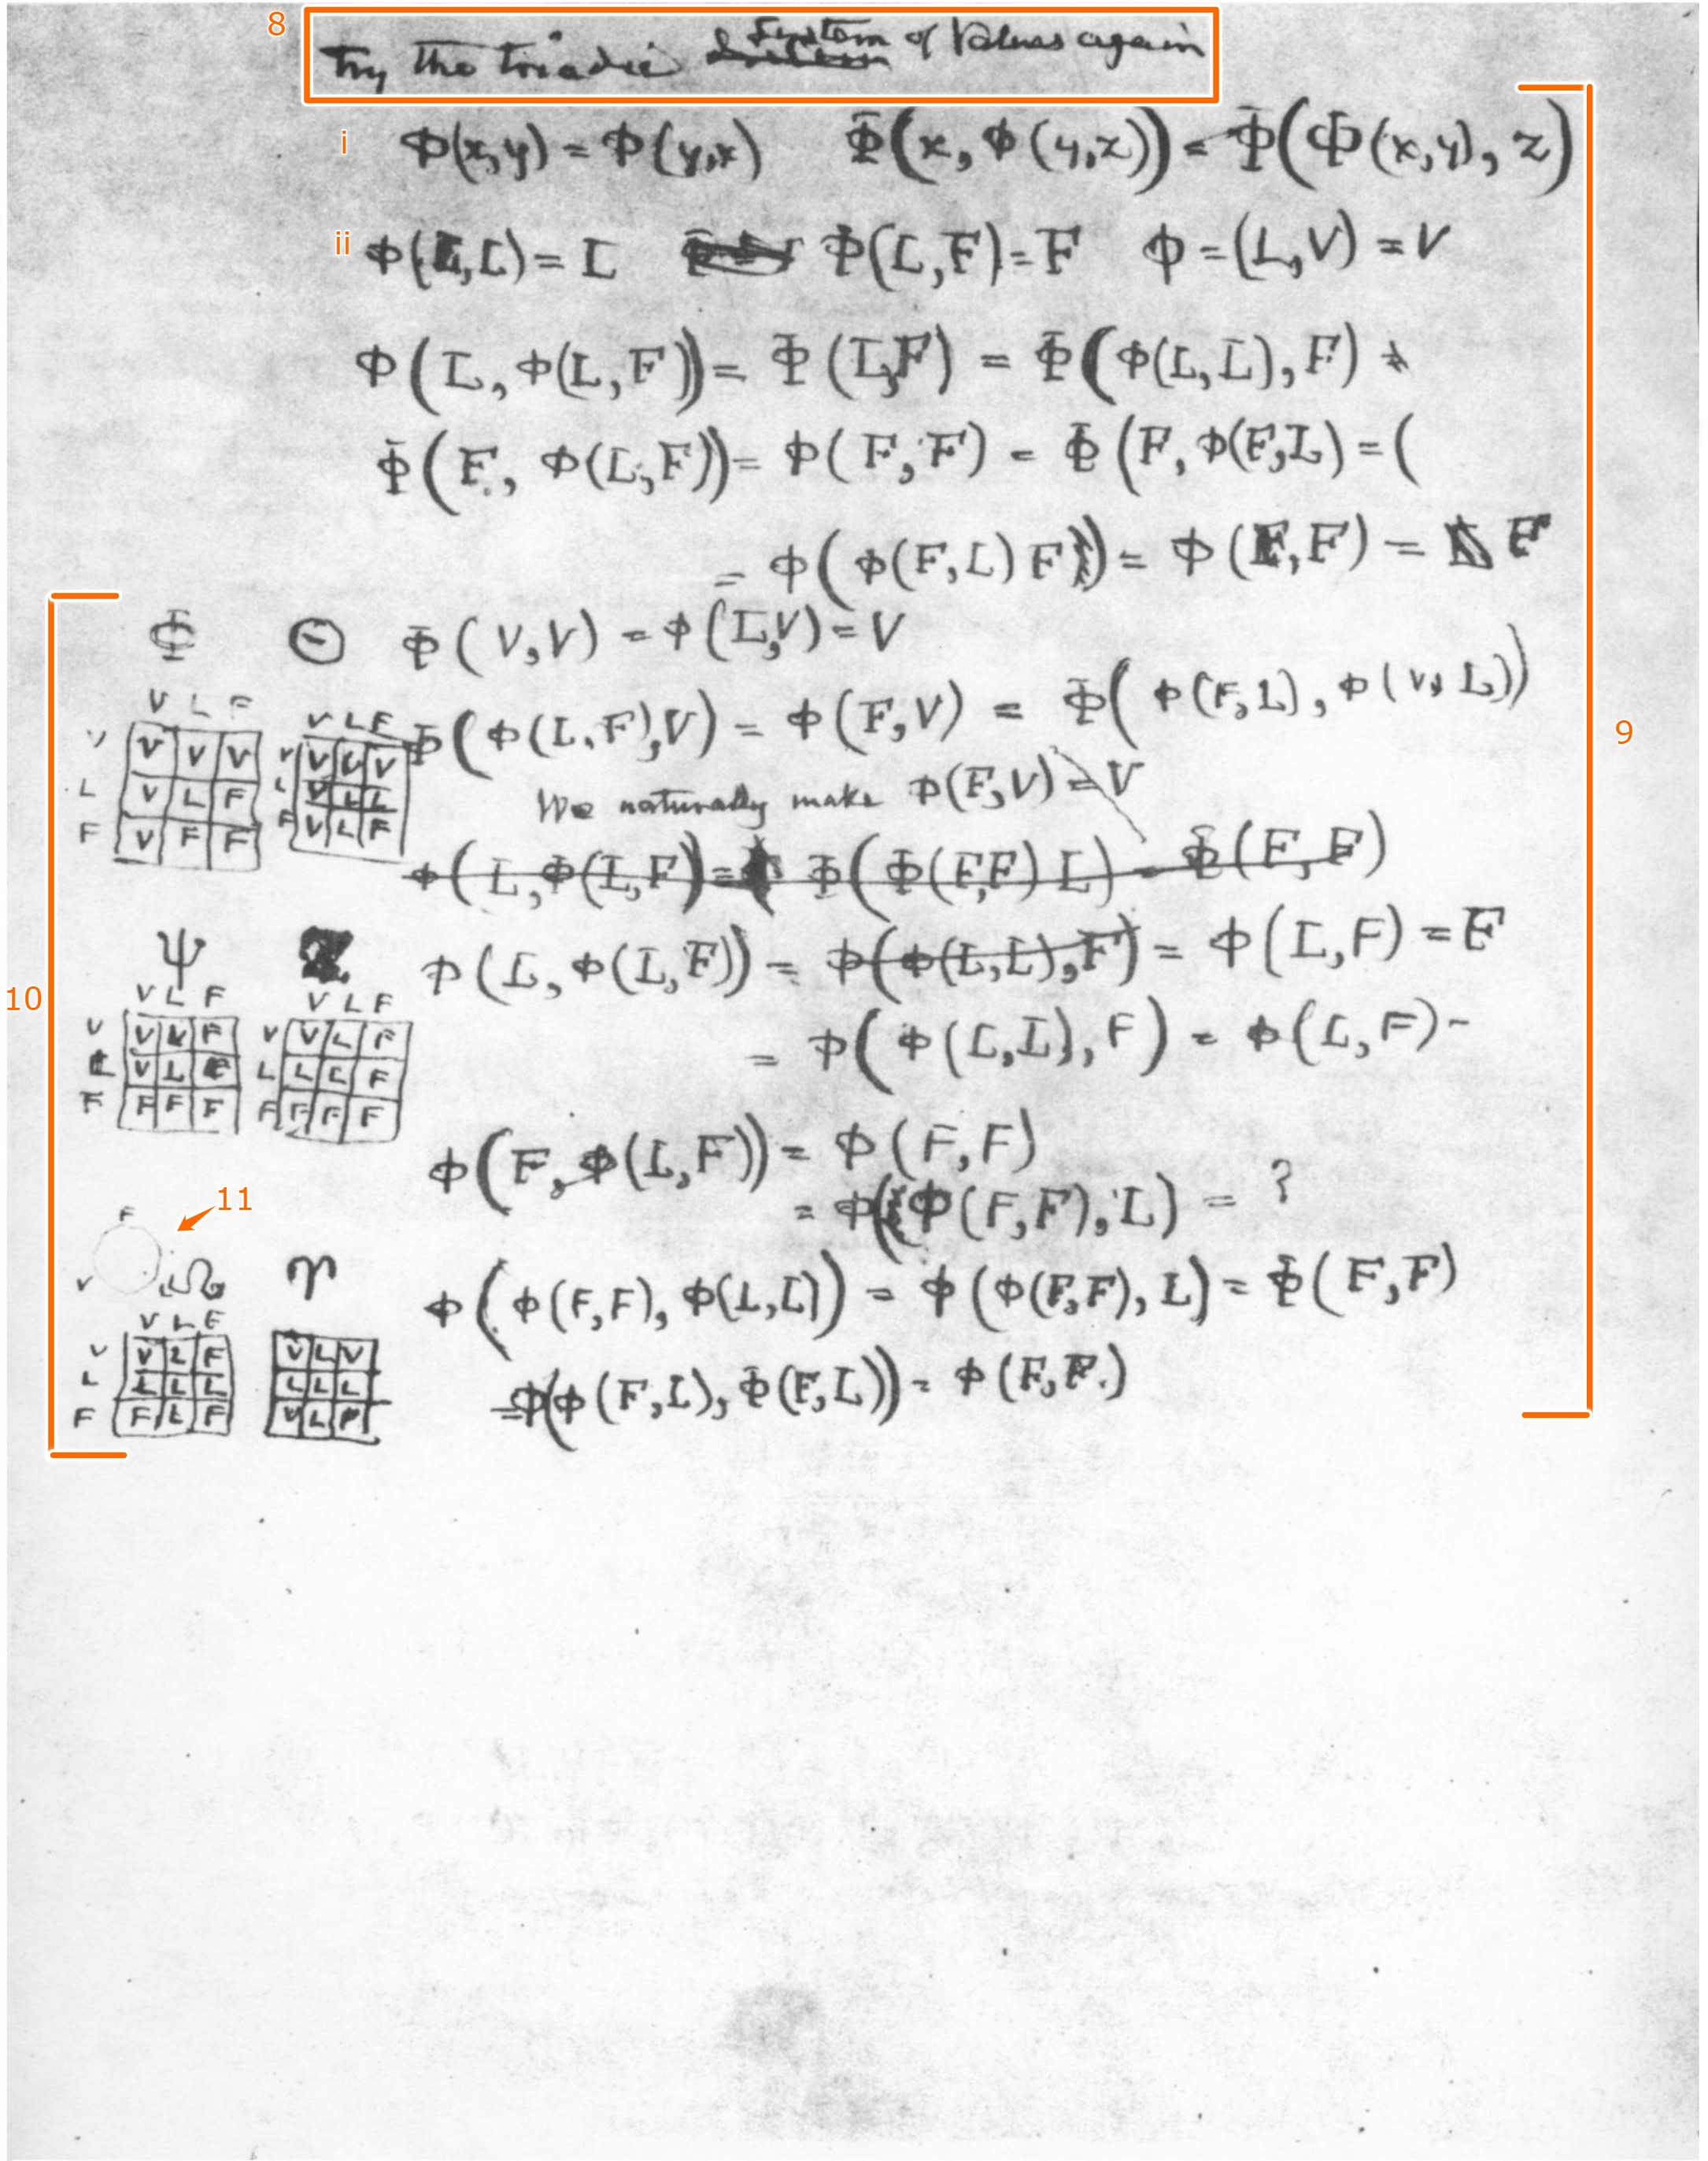
\includegraphics[width=\textwidth]{images/page two.jpeg}
    \caption{Second Page, \href{https://iiif.lib.harvard.edu/manifests/view/drs:15255301$640i}{seq. 640 V.}}
    \label{fig:640}
\end{figure}

The second page appears to have been far more successful. At the top of the page (8) is written ``try the triadic system of values again.'' Below the word `system', `definition' appears crossed out.

The bulk of the page (9) appears to be devoted to working out the semantics of $\Phi$. On the first line (i) two formulae appear, indicating that $\Phi$ is both commutative and associative. Line two (ii) gives valuations for $\Phi$ when paired with $L$ and any value. In lines 3, 4, and 5, the formulae in (ii) are slotted in either place of $\Phi$ and are identified with other combinations. The rest of (9) amounts to more of the same. Given that all that Peirce had worked out for $\Phi$ in the main body of the page is consistent with its characteristic matrix on the left, it seems reasonable to conclude that the main goal here was to give this definition. It seems he was successful in these regards as well.
\begin{displaymath}
\begin{array}{|c c|c|c|}
% |c c|c| means that there are three columns in the table and
% a vertical bar ’|’ will be printed on the left and right borders,
% and between the second and the third columns.
% The letter ’c’ means the value will be centered within the column,
% letter ’l’, left-aligned, and ’r’, right-aligned.
p & q & \Phi(p, q) & \Psi(p, q)\\ % Use & to separate the columns
\hline % Put a horizontal line between the table header and the rest.
V & V & V & V\\
V & L & V & V\\
V & F & V & F\\
L & V & V & V\\
L & L & L & L\\
L & F & F & F\\
F & V & V & F\\
F & L & F & F\\
F & F & F & F\\
\end{array}
\end{displaymath}

One curiosity resulting from this is that in the marginal note (10) we find not one, but six operators with characteristic matrices. It is not immediately clear where all of the other operators came from. While it is certainly possible that he had worked these out on other pages that have since been lost, it is also possible that one operator was all he needed to work out the others. This would not be totally uncharacteristic of Peirce as he had earlier shown, in MS 378, that all boolean operators could be built up from combining $\lnot$ and $\lor$ into a single logical operator, which we now call `nor' (CP 4.12-20, from an untitled paper written in 1880). So, it seems possible that once he had a consistent definition of $\Phi$ worked out, he was able to discover the rest of the operators by combining $\Phi$ with the negations he worked out on the previous page. This idea is somewhat supported by the complex network of morphisms between the operators that Turquette discovered \citep{turquette_dualism_1972}. Every one of Peirce's operators is the dual of some other with respect to the $\bar{\lnot}x$ negation ---where an operator $O$ is the dual of another $O^{*}$ with repect to a negation $\lnot^{i}$ just in case $\lnot^{i}(\lnot^{i}p O \lnot^{i}q)\equiv (p O^{*} q)$--- like $\land$ and $\lor$ in classical logic. For example, $\Phi$ is the dual of the $\Psi$ operator immediately below it with respect to $\bar{\lnot}x$. In the same fashion, $\Theta$ and $Z$ are duals, and so are $\Omega$ and $\Upsilon$. 

Another layer of depth in this network of relations can be appreciated if we consider the cyclical total negations Peirce gave on the first page. For any one of the operators on the page there is a tri-morphism ---where an operator $O$ has $O^{*}$ and $O^{'}$ as trimorphs with respect to a cyclical negation $\mathring{\lnot}$ just in case $(pOq\equiv \mathring{\lnot}(\mathring{\lnot}pO^{*}\mathring{\lnot}q))\land (pOq\equiv \mathring{\lnot}\mathring{\lnot}(\mathring{\lnot}\mathring{\lnot}pO^{'}\mathring{\lnot}\mathring{\lnot}q))$ holds between $O$ and the other two operators. For example $p\Phi q$ is equivalent to both $\diagdown{}(\diagdown{p}Z\diagdown{q})$--- and $\diagup{}(\diagup{p}\Upsilon \diagup{q})$. It turns out that in the six operators defined in the margin, there are two trimorphisms. While $\Phi, Z$ and $\Upsilon$ are trimorphs of each other, so are $\Psi, \Theta$ and $\Omega$.

There is some textual evidence Turquette points out to support the idea that Peirce was aware of this relationship \citep{turquette_dualism_1972}. If we look closely to the left of $\Omega$ (11), there appears to be a small circle with $V, L$ and $F$ around the perimeter about 120 degrees apart from one another. Moving clockwise around the circle appears to correspond with the $\diagdown{x}$ negation ($\diagdown{V}=F, \diagdown{F}=L,$ and $\diagdown{L}=V$). Moving counterclockwise corresponds to the $\diagup{x}$ negation ($\diagup{V}=L, \diagup{L}=F,$ and $\diagup{L}=V$). This may suggest, as Turquette claims, that Peirce was aware of these trimorphisms and was experimenting with his cyclical negations while developing his operators.

Even more dualisms can be found if we consider negations other than the ones Peirce gave, as Turquette has also shown. However, restricting ourselves only t0 the negations Peirce treated in these notes, we can draw the following network of relations between his operators:


% https://tikzcd.yichuanshen.de/#N4Igdg9gJgpgziAXAbVABwnAlgFyxMJZABgBpiBdUkANwEMAbAVxiRAB12AFACyxAC+pdJlz5CKAEzkqtRizacAKjxg46g4SAzY8BImQCMs+s1aIO3bJpG7xRaceqmFFgFo3tovRJKlJJvLmlgDyALYwAOYaQrZi+lL+gWaK7ACqaNgM+gKyMFCR8ESgAGYAThBhSGQgOBBI0iAMdABGMAxc3vYWWGDYsCDOQaktdGXAAB4CgyCqdFBskGCs1HB8JTjV1Ay9wXAQOwvU6lgMiwQrIG1gC4jEsSDllUiGx-WIAMxDKRaco+NTGZzW7gC4zZptDpdBIgXr9S7XW73LRPKqIAAsbyQAFZvq5LP9JtNtq12p07DC4VgBtRgedljNEdUHqitrV3l85D9LJEynQaDAieDSVCKRImjANoyYDdmSiKmjOXUcSTIeT4uKGJLNnjgpxefzBYDqEy7iyFSr2WyXHr2AaBULVWToeKylhIjwdVcZUjzc9EK8rYhGhDnWK2G6PV7TTUbal7Ubpn60Y1lRjdfG+Q7jU0ReqfBH3Z7PKz00HA6HRRq2FqpRnfnas4nBBQBEA
\[
\begin{tikzcd}
\Phi \arrow[d, "\bar{x}" description, no head] \arrow[rrd, "\diagdown{x}"]     &  & \Theta \arrow[d, "\bar{x}" description, no head] \arrow[lld, "\diagdown{x}"'] \\
\Psi \arrow[d, "\diagdown{x}"']                                                &  & Z \arrow[d, "\diagdown{x}"]                                                   \\
\Omega \arrow[rr, "\bar{x}" description, no head] \arrow[rruu, "\diagdown{x}"] &  & \Upsilon \arrow[lluu, "\diagdown{x}"']                                       
\end{tikzcd}
%\begin{tikzcd}[row sep=large,column sep=large]
%\Phi \arrow[d, ''\bar{x}'' description, no head] \arrow[rrd, ''\diagdown{x}'']     &  & \Theta \arrow[d, ''\bar{x}'' description, no head] \arrow[lld, ''\diagdown{x}'''] \\
%\Psi \arrow[d, ''\diagdown{x}''']                                                &  & Z \arrow[d, ''\diagdown{x}'']                                                   \\
%\Omega \arrow[rr, ''\bar{x}'' description, no head] \arrow[rruu, ''\diagdown{x}''] &  & \Upsilon \arrow[lluu, ''\diagdown{x}''']                                       \end{tikzcd}
\]
In the diagram the lines without arrowheads that are separated by $\bar{\lnot}x$ in the middle mark the dualisms. The directional arrows mark the $\diagdown{x}$ trimorphisms. If the direction of the arrows is reversed the $\diagup{x}$ trimorphisms can be observed. These considerations may offer a possible explanation for how Peirce got the full set of operators after seemingly only defining $\Phi$. For example, from $\Phi$ he could have worked out its $\bar{\lnot}x$ dual, $\Psi$. From there he could have worked the rest out by applying either $\diagdown{x}$ or $\diagup{x}$ to these two to unveil each of their trimorphs.\footnote{For further discussion on the relationships between Peirce's triadic operators and to see how they can be used to make a sound and complete logic under different axiom sets and with the addition of quantification, see \cite{turquette_peirces_1967, turquette_storrs_1968, turquette_peirces_1969, turquette_minimal_1976, turquette_alternative_1978, turquette_quantification_1981, turquette_defining_1988}} However, the textual evidence is so small that concluding as such would be a bit of a leap.

Each of Peirce's operators also has an analogue in more familiar modern systems of three-valued logic. The most familiar of these are $Z$ and $\Theta$, which are the versions of conjunction and disjunction in Łukasiewicz's system as well as Kleene's strong conjunction and disjunction (\citeyear{kleene_introduction_1952}, 327-336). $\Upsilon$ corresponds to a connective used by Bochvar as well as Kleene's weak disjunction \citep{bochvar_three_1939}. Likewise, $\Omega$ corresponds to another of Bochvar's connectives and Kleene's weak conjunction. $\Phi$ and $\Psi$ are probably the most obscure of these operators. They appear as disjunction and conjunction respectively in a system developed by Sobocinski \citeyearpar{sobocinski_axiomatization_1952} as well as in Coopers ``logic of ordinary discourse'' \citeyearpar{cooper_propositional_1968} which was pointed out by R. Z. Parks \citeyearpar{parks_mystery_1971}.\footnote{For more connections between Peirce's three-valued operators and more recent works, see \cite{lane_2001}.}

It may also be worth noting that Turquette has proven that any one of Peirce's operators along with either one of the cyclical negations can form an expressively complete system. Extrapolating on this work further to suggest what Peirce's definition of implication, Turquette was also able to develop a sound and complete axiomatic system of three-valued propositional logic with one inference rule.
%maybe watch video. it's going to take a few more sentences here.

Another interesting curiosity is that all of Peirce's operators seem to be versions of conjunctions and disjunctions, and he seems to have shown little interest in asymmetric relations, like conditionals. So, why was Peirce so preoccupied with these kinds of operators? This possibly has to do with the kinds of things he was hoping to represent within this system. It is also possible that he was not sure how he wished to define a conditional operator for his triadic logic. This doesn't seem to have stopped him with regard to conjunction or disjunction, as he appeared to be content to have multiple forms of these.

\section{seq. 645 R.}

\begin{figure}
    \centering
    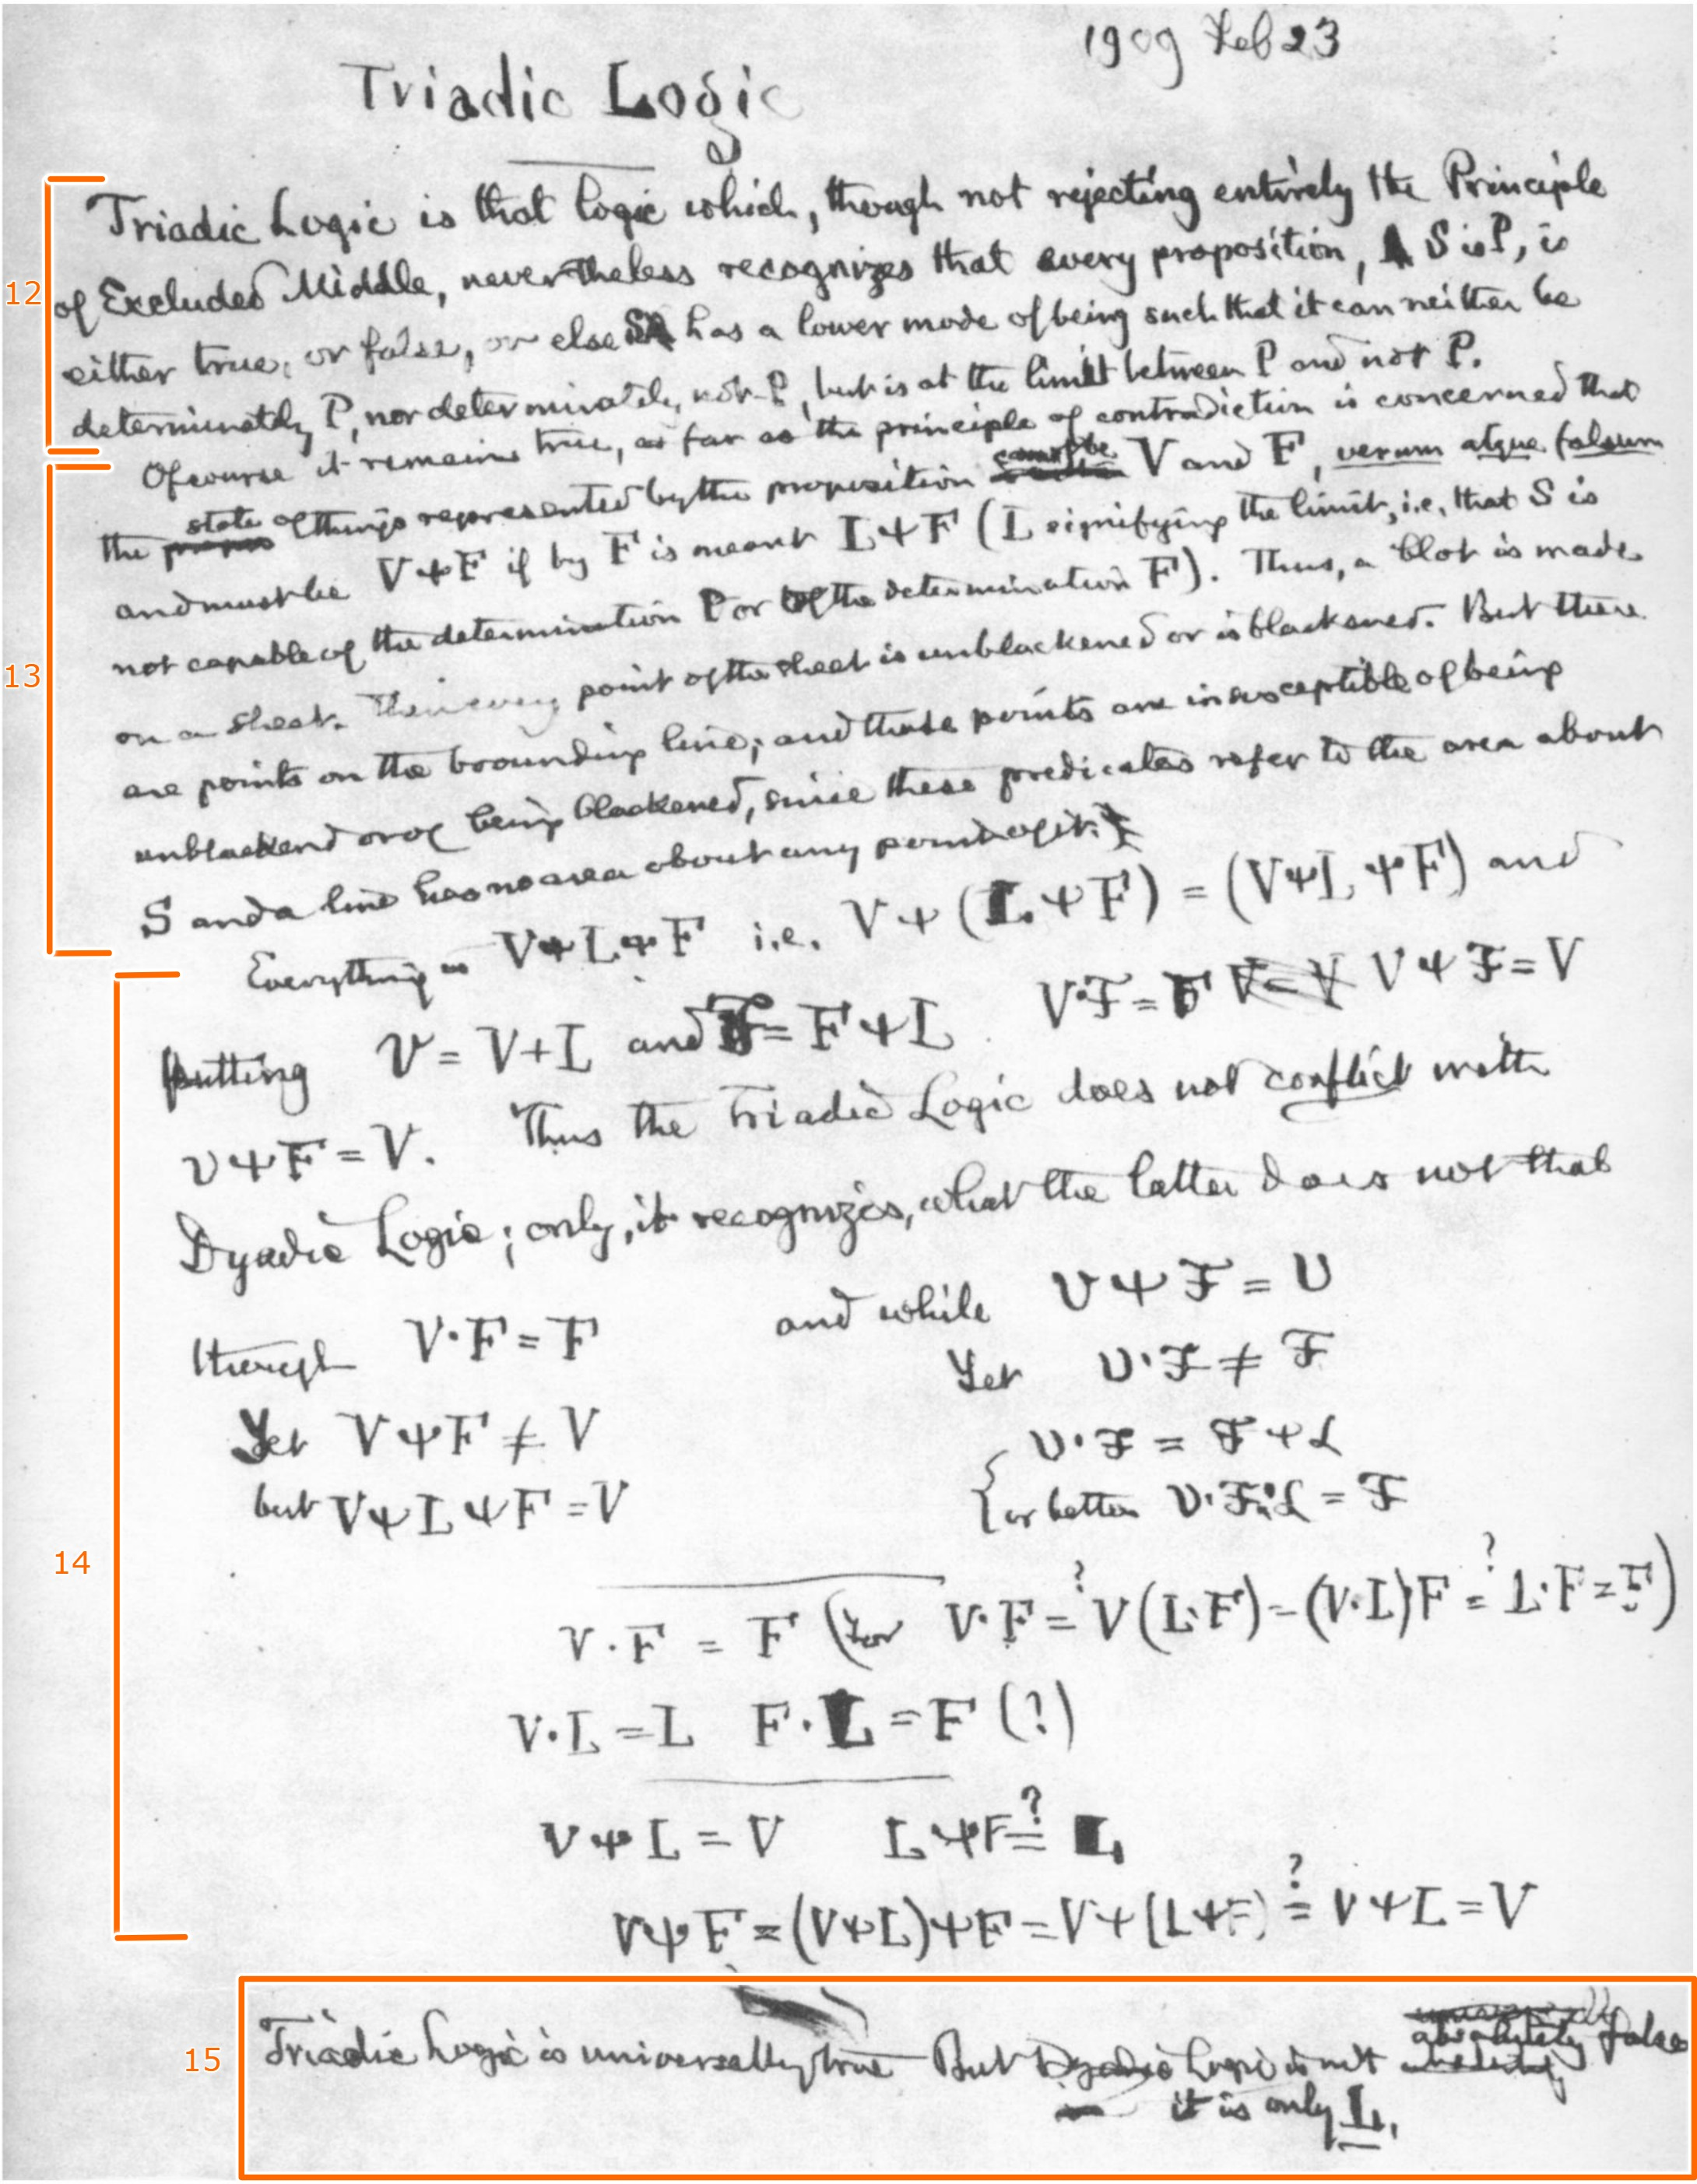
\includegraphics[width=\textwidth]{images/page three.jpeg}
    \caption{Third Page, \href{https://iiif.lib.harvard.edu/manifests/view/drs:15255301$645i}{seq. 645 R.}}
    \label{fig:645}
\end{figure}

The third and final page is the most substantive in terms of textual evidence for exactly what Peirce was trying to accomplish with his three-valued semantics. In it we find a description of triadic logic along with a rather bizarre example of the sorts of things he intended $L$ to apply to. The page is titled ``Triadic Logic'' and is dated February 23, 1909. 

The text (12) begins: \begin{quotation}\noindent``Triadic logic is that logic which, though not rejecting entirely the principle of excluded middle, nevertheless recognizes that every proposition, S is P, is either true or false, or else S has a lower mode of being such that it can neither be determinately P, nor determinately not P, but is at the limit between P and not P.''\end{quotation} This passage will be important for my later analysis. He does not mention here what he means by `mode of being' but this notion figures importantly in his philosophy elsewhere. To explain this notion requires a brief foray into an aspect of Peirce's thought I have referred to as his triadism: his penchant for making tripartite divisions in philosophy.  Peirce developed a concept of three Universal\footnote{He seems to have thought of these categories as being of higher order than even metaphysical categories.} Categories that he used in his analysis of all philosophical ideas. He sometimes calls them categories of being, sometimes of ideas, of thoughts, and of nature (or `things' as he usually says). Depending on the subject matter, these categories will have different names, but in the most abstract sense they are always the same. In his 1904 letters to Lady Welby, he defines these categories as follows:
\begin{quotation}
\noindent``Firstness is the mode of being of that which is such as it is, positively and without reference to anything else.

Secondness is the mode of being of that which is such as it is, with respect to a second but regardless of any third.

Thirdness is the mode of being of that which is such as it is, in bringing a second and third into relation to each other.'' (CP 8.328)
\end{quotation}
 In the abstract, the categories are firsts (things that are what they are without reference to anything else), seconds (things that exist only in reference or connection something else), and thirds (which exist in bringing together a second and a third). An example of the sort of thing that would be a first for Peirce is a quality, like a color. There is some sense in which colors exist without reference to anything else. We all have a concept of `redness' that we can think of independently of red objects. So the color red is a first. Seconds are like particular objects, like a red blanket. A red blanket is what it is in reference to two things: being red and being a blanket. Thirds do not lend themselves to simple examples as easily, and are more recognizable within the various contexts Peirce applies his categories. He sometimes calls them laws, sometimes reasons, and other times powers.

Having some idea of Peirce's categories, we can now examine his three modes of being. Each of the objects that falls into his three categories has an associated mode of being: ``My view is that there are three modes of being. I hold that we can directly observe them in elements of whatever is at any time before the mind in any way. They are the being of positive qualitative possibility, the being of actual fact, and the being of law that will govern facts in the future'' (CP 1.23). So, firsts, being merely qualities, have the mode of being of a possibility. This is because they do not exist on their own except for in the possibility that they are instantiated by some object, in the sense that the color red does not really exist independently of red objects. Seconds, have the mode of being of actuality. These are ordinary objects that occur in the world around us. All the objects that we normally see and interact with are seconds. Thirds have the mode of being of necessity. Again, this notion is much more difficult to understand as precisely as the first two. The things that are thirds for Peirce can loosely be understood as laws of nature. They are basically general facts about seconds. He says ``This mode of being which \textit{consists}, mind my word if you please, the mode of being which \textit{consists} in the fact that future facts of Secondness will take on a determinate general character, I call a Thirdness'' (CP 1.26). Part of the difficulty with understanding and stating precisely what thirds are is thinking of them as objects. We do not normally think of laws as objects. Nonetheless, suppose that every time a diamond is dragged across a pane of glass, from now into the indefinite future, a scratch is produced. Then the third in this case is the law or fact of the universe that determines that all diamonds scratch all panes of glass.

Having cleared up Peirce's categories and modes of being, it is already clear that modality was built in to these notions. When Peirce discusses triadic modality, as well as when Fisch and Turquette, Lane, and I do so, it is the possibility, actuality, and necessity built into these modes of being that we are referring to. So when Peirce refers to ``modes of being'' in his logic notebook, there is clearly some sense in which modality is involved.

The note goes on to say (13) ``Of course it remains true, as far as the principle of contradiction is concerned that the state of things represented by the proposition cannot be $V$ and $F$, \textit{verum atque falsum} and must be $V+F$ if by $F$ is meant $L+F$ ($L$ signifying the limit, i.e. that S is not capable of the determination P or of the determination $F$).''\footnote{When Peirce uses $+$ in this way, it is just a notational variant of $\lor$.} Peirce's strange example then follows: ``Thus, a blot is made on a sheet. Then every point of the sheet is unblackened or blackened. But there are points on the boundary line; and those points are insusceptible of being blackened or of being unblackened, since these predicates refer to the area about S and a line has no area about any point of it.'' 

At first glance this seems to be an example of a category mistake. The proposition `point $x$ on the boundary line is blackened' should apparently take the value $L$, because $x$ would have to have area in order to be blackened or unblackened, and points on lines do not have area. Thus, this predicate is undefined for $x$. The strange thing is that points themselves do not have any area, which runs contrary to Peirce's claim that ``every point of the sheet is blackened or unblackened.'' Another possible interpretation is that he thought that the properties of a point were determined by the properties of the immediate area surrounding the point. This view would make more sense, as the points on the boundary line really would be neither fully blackened nor unblackened, because the immediate area surrounding them would be both. But it is unclear from this passage alone whether this interpretation is accurate. At face value, it is also unclear how this example is supposed to relate to Peirce's earlier comment about modes of being. As far as examples go, this one is not very enlightening. It turns out that the example actually pertains to Peirce's theory of continuity, as Lane argues \citeyearpar{lane_peirces_1999}. 

The bulk of the rest of the page (14) contain Peirce's metalogical observations about triadic logic and traditional two valued logic. The sentence in the middle reads ``Thus the triadic logic does not conflict with dyadic logic; only it recognizes what the latter does not, that though...'' and then he uses formulae to demonstrate this lack of conflict.

At the bottom of the page (15) we find Peirce triumphantly declaring ``Triadic logic is universally true. But Dyadic Logic is not absolutely false, it is only $L$.'' So it seems Peirce was trying to extend dyadic logic rather than completely revise it.

\section{seq. 637 R.}

\begin{figure}
\centering
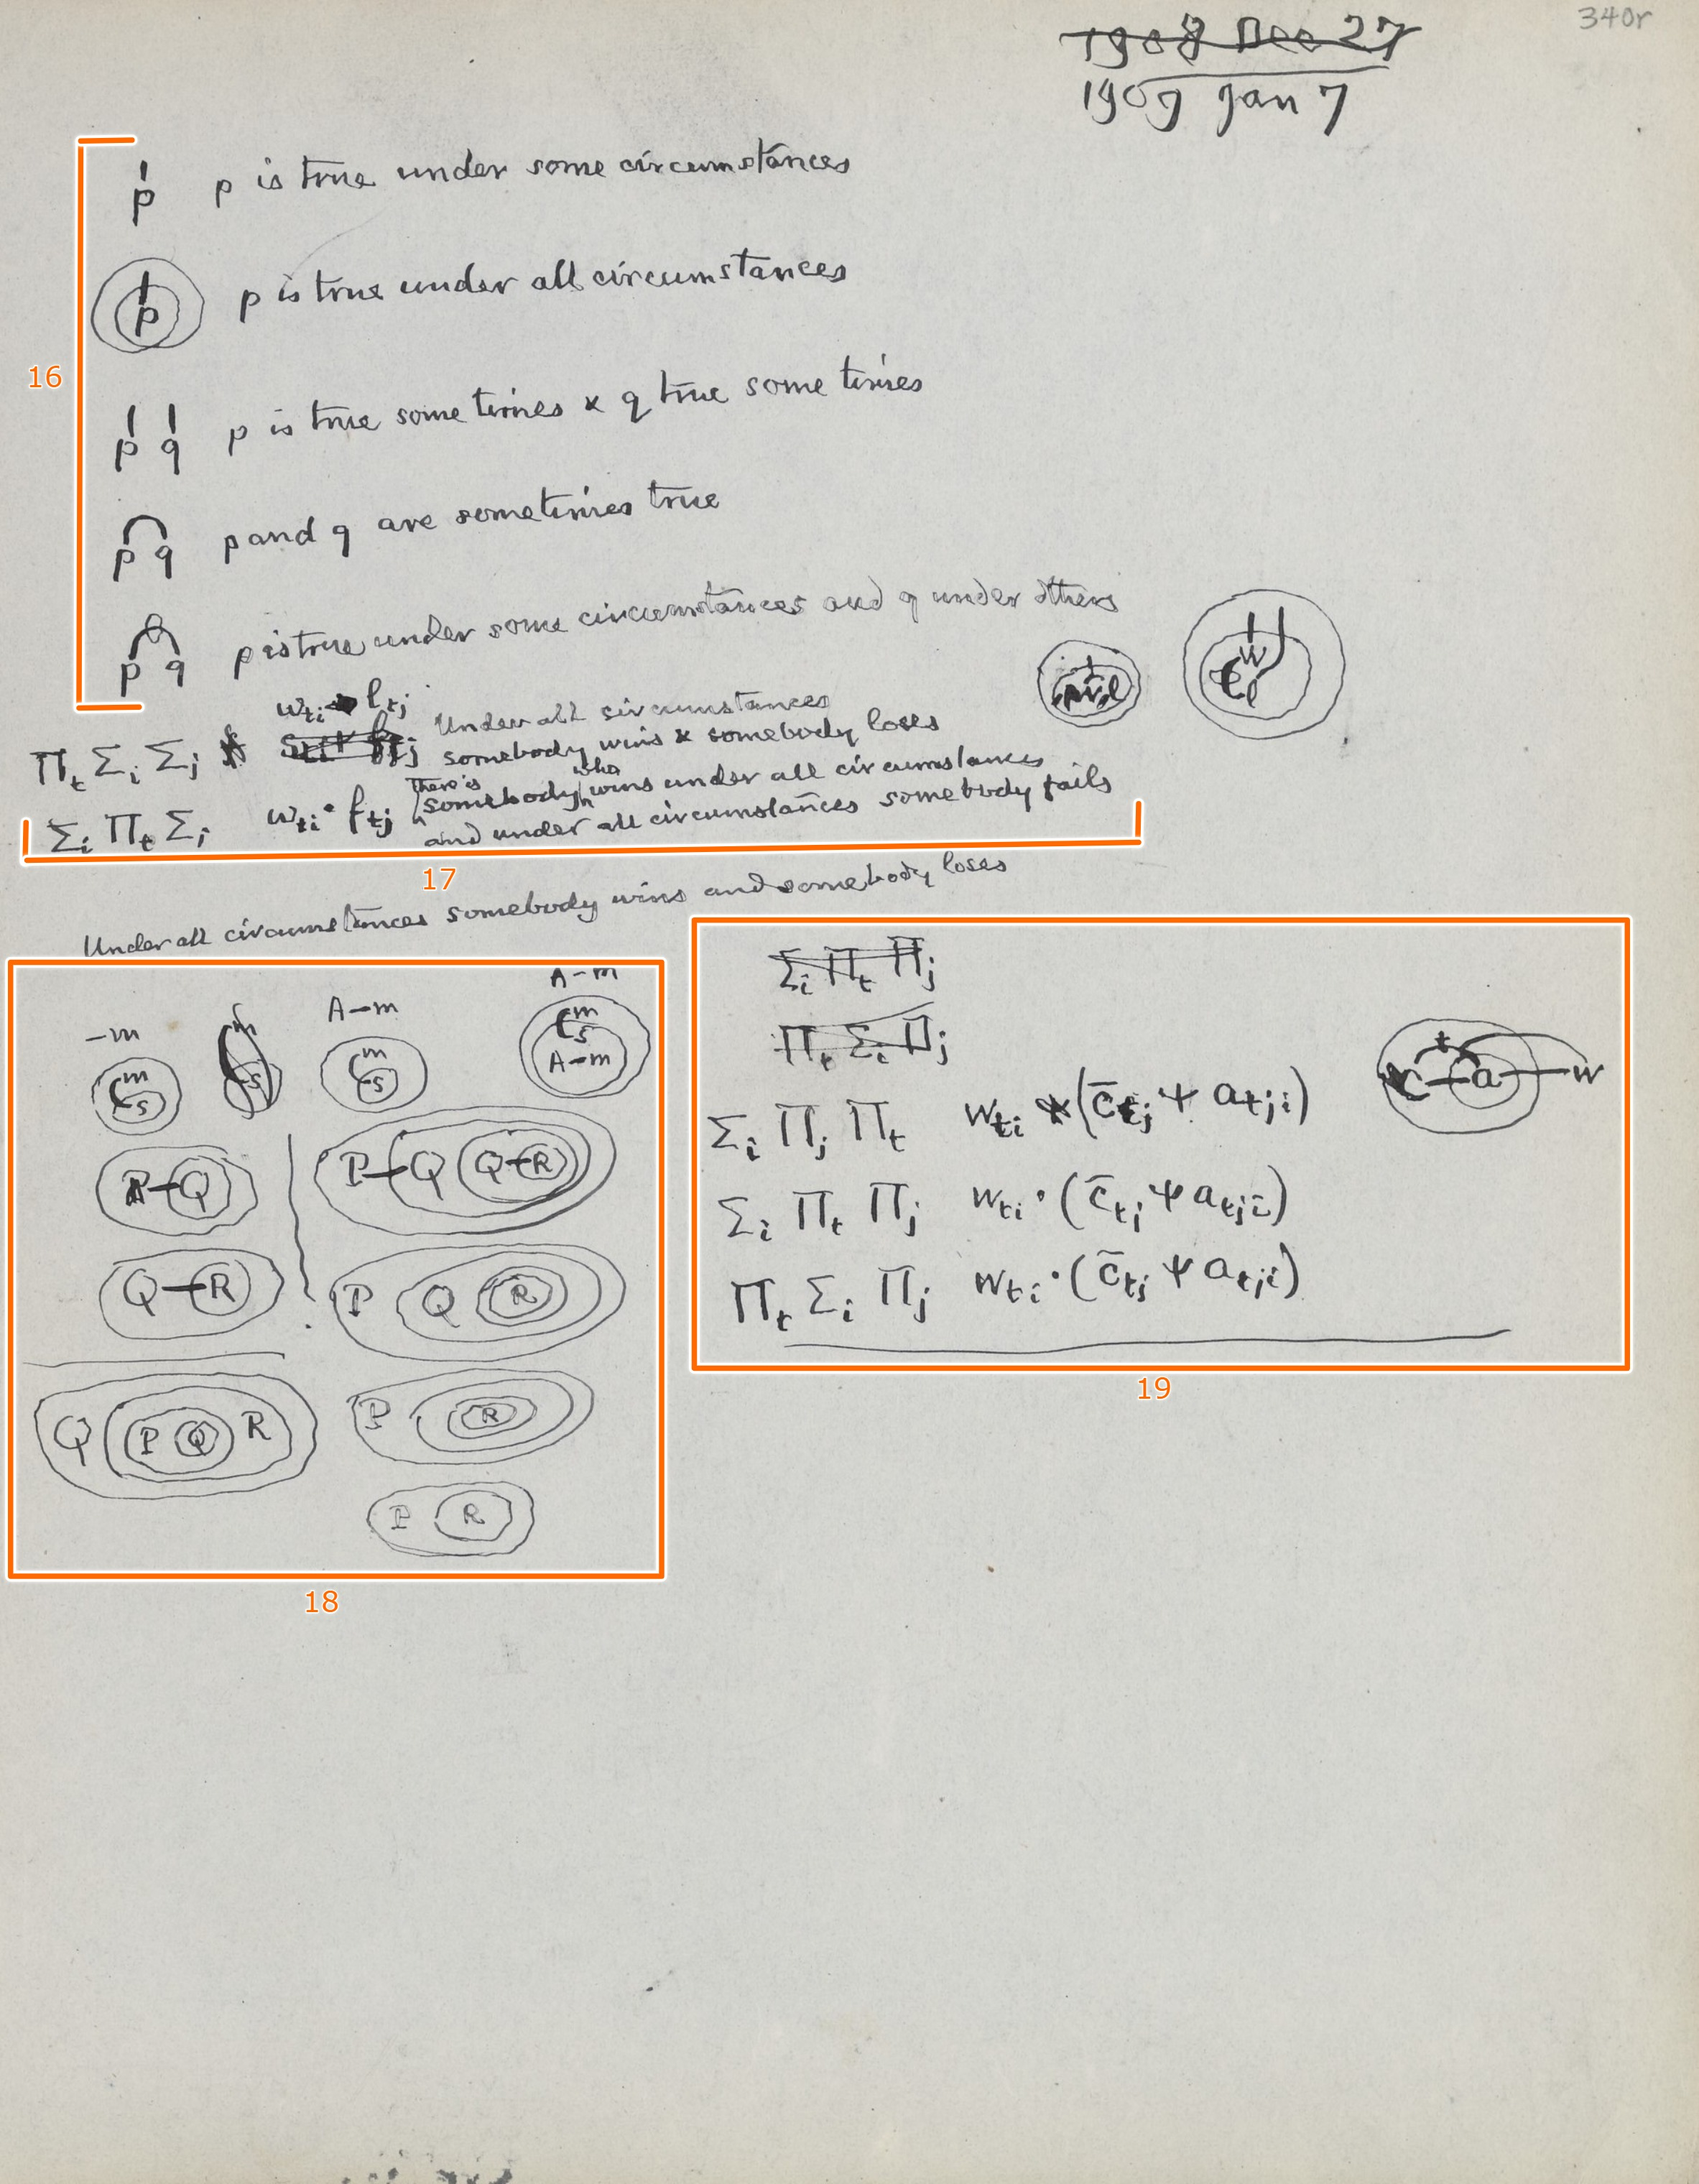
\includegraphics[width=\textwidth]{images/seq637.jpeg}
\caption{seq. 637 R.}
\label{fig:seq637}
\end{figure}

The first page preceding those that Fisch and Turquette take note of might also have some close philosophical connections to Peirce's triadic logic. In it, Peirce appears to be attempting to introduce some kind of modal operator to his already established system of existential graphs.\footnote{Peirce's discussion of existential graphs can be found in CP 4.347--584. See also \cite{roberts_existential_2009}, \cite{shin_iconic_2002}, and \cite{hammer_semantics_1998}.} Not all of the material on this page is expressed in existential graphs. On the same page, Peirce also uses algebraic notation. Fisch and Turquette do mention this page in their discussion but they tell us nothing of what is on it except that the December 27th, 1908 date has been crossed out and replaced with January 7th, 1909.

 The operator Peirce is introducing is a vertical line attached to a proposition $p$. When it is fixed to an atomic proposition, $p$, it asserts (16) ``$p$ is true under some circumstances.'' Thus, the dash appearing above $p$ on the page seems to be roughly analogous to the usual modal operator $\Diamond$. The next line shows us how to use this operator to say that a proposition is necessary. The graph to the left of this line can be translated as $\lnot \Diamond \lnot p$.\footnote{ Peirce's existential graphs are expressed using only two or three operations as long as the system is propositional or first order. For propositional logic, a closed curve indicates its contents are being negated and the juxtaposition of two formulae together indicates conjunction. For the first order system the only addition is the line of identity which operates on formulae as an existential quantifier does. Interestingly though, there were systems that were designed to treat modal propositions as well as higher order propositions. These included additional operators.} In the next line Peirce show us how to symbolize ``$p$ is true sometimes and $q$ is true sometimes.'' The lines above $p$ and $q$ in the last example can be joined to assert the conjunction of $p$ and $q$ is possible: ``$p$ and $q$ are sometimes true.'' When the joined line has an ellipse running through it, this means ``$p$ is true under some circumstances and $q$ under others.'' This would presumably mean something similar to the modal formula, $\Diamond \lnot (p \land q)$.
 
 Immediately below (17), Peirce has written some first order formulae and the English sentences these are meant to symbolize. He uses $\Pi$ and $\Sigma$ as symbols for universal and existential quantification respectively. This is nothing new as he had been using these symbols since at least 1885 when he published a paper about adding quantifiers to the already familiar set of Boolean operators \citep{peirce_algebra_1880}. The subscripts attached to the quantifiers are the variables to which they are bound. It is unclear what the connective in the first formula is but it appears to be a crossed out $\Psi$. The formula is $\Pi_{t} \Sigma_{i} \Sigma_{j} w_{ti} \xcancel{\Psi} l_{tj}$ and we are told this means ``Under all circumstances somebody wins and somebody loses.'' The next formula reads $\Sigma_{j} \Pi_{t} \Sigma_{i} w_{ti} \cdot f_{tj}$ which is interpreted as ``There is somebody who wins under all circumstances and under all circumstances somebody fails.'' For both of these formulae, the $t$ variable seems to be ranging over 'circumstances' while $i$ and $j$ range over people. Written immediately below, (17) the note says ``Under all circumstances somebody wins and somebody loses.''

Among other oddities on this page, it is unclear exactly what this example has to do with the material in the previous discussion. In the previous portion Peirce seems to be interpreting his new operator as asserting something like contingency. But there may be difficulties with this interpretation as he only states that the $p$ with a dash on top of it asserts that there are some circumstances in which $p$ is true, while contingency would require that it sometimes be false as well. This lends weight to the interpretation that regards $p$ with a dash as possible rather than contingent. A `possible' proposition would be true as long as there is at least one set of `circumstances' in which it is true. Contingency would require at least one false set as well. However, neither of these interpretations help to explain the choice of `winning,' `losing' or `failing' as an example of the kind of propositions Peirce was targeting. There is one plausible explanation though, that might lend evidence to this pages connection with Peirce's triadic logic. This is the unmentioned possibility of a `tie.' The reason Peirce may have chosen games as an example here is because there is a third possible circumstance that is often overlooked when we talk about games. This also might explain why there is no `tie' predicate on the page. If there were an additional truth value, then there would be no need for this additional predicate. The possibility of a tie would be built into the system. One might object that the second formula wouldn't make sense under this interpretation. However, that might have been the point, and this could have been a counterexample to the classical interpretation of conjunction. Another possibility is that $\cdot$ is interpreted differently in this situation, in such a way that the conjunction of middle valued statements would yield true.

At the bottom of the page, on the left (18), we can see more examples of existential graphs however the operator in the upper portion of the page makes no appearance. The lines and curves that can be observed are called ``lines of identity'' and they are used to express quantification within the system. The first three graphs from left to right in (18) involve lower case $m$ and $s$, which may refer to individuals, and an upper case $A$, which may be a predicate. Since they make no appearance in the text in the upper portions of the page, it is difficult to say how they are to be interpreted. The first graph can be translated as $\exists x m(x) \land \exists x (m(x) \lif s(x))$. The second: $\exists x(A(x) \land m(x)) \land \exists x (m(x) \lif s(x))$. The third: $\exists x (A(x) \land m(x)) \land \exists x (m(x)\lif (s(x) \land \exists y( A(y) \land m(x))))$. The rest of the graphs in this portion involve metavariables $P$, $Q$, and $R$, so Peirce probably did not have any specific interpretations in mind. One graph is boxed off from another series of graphs. The unboxed series appears to illustrate Peirce's erasure rules for his existential graphs, which are basically kinds of inference rules.

To the right (19) appears more symbolic first order formulae in which $\Psi$ makes another appearance. The `wins' predicate is involved again as well as two undisclosed predicates symbolized by `$c$' and `$a$'. A natural interpretation of `$c$' would be that it has something to do with `circumstances.' It is unclear what `$a$' is meant to be aside from a three-place predicate. The formulae are as follows:
\begin{gather*}
\Sigma_{i} \Pi_{j} \Pi_{t} w_{ti} \xcancel{\peirceor} (\bar{c}_{tj} \Psi a_{tji}) \\
 \Sigma_{i} \Pi_{t} \Pi_{j} w_{ti} \cdot (\bar{c}_{ti} \Psi a_{tij}) \\
  \Pi_{t} \Sigma_{i} \Pi_{j} w_{ti} \cdot (\bar{c}_{tj} \Psi a_{tij})
\end{gather*}
The first $\peirceor$ is crossed out presumably because Peirce meant to use the classical conjunction. Since there is no indication of what `$a$' is meant to be interpreted as, and there is no characteristic matrix given for $\Psi$ at this point, it is difficult to say what the significance of this is.

At this point I would like to raise an interesting question in connection with Peirce's existential graphs and his triadic logic. Peirce was exceedingly proud of his existential graphs, lovingly referring to them as his ``chef d'oeuvre.'' In 1903 he expressed his preference for them over his previous algebraic approach, calling them ``far more perfect'' with regards to understanding necessary reasoning (CP 4.429). Why then, if Peirce so admired and preferred his diagrammatic system, does he return to the algebraic approach when developing his triadic logic years after he was satisfied with existential graphs? His choice is odd not only because of his preference for this system but also because he had developed a system of graphs for dealing with modal propositions: the gamma graphs (CP 4.510-529 and 573-584). This may provide evidence that Peirce was not concerned with modality when developing his triadic logic, or at least not the kind of modality dealt with by his gamma graphs.

The mix of algebraic expressions and graphs on this page might be evidence that Peirce was trying to develop a graphical system capable of dealing with whatever was at issue, but that he failed to work this out to his satisfaction and reverted to his former approach. The likely explanation for this decision has to do with how logical notions like validity are given for his graphs. In the system of existential graphs (henceforth EG), deductive validity is defined syntactically according to the rules of the system, where as the algebraic approach defines validity semantically. As such, there are no characteristic matrices given for the operators of EG, nor is there any discussion of truth values when Peirce sets up the system. This would make it difficult to work with if the subject matter of interest required the admission of a third truth value and would likely require additional rules and operators. It might be easier to start with the algebraic approach and then formulate modified rules for EG after the system is better understood.

It is worth noting, that while the gamma portion of EG does provide some resources for reasoning about modalities and the like, it was the most undeveloped part of the system and Peirce was never quite satisfied by it. Referring to the gamma portion in connection with the first order and propositional system, Peirce writes: \begin{quotation} \noindent``Generally speaking [the propositional and first order portions are] unable to reason about abstractions. It cannot reason for example about qualities nor about relations as subjects to be reasoned about. It cannot reason about ideas. It is to supply that defect that the gamma part of the subject has been invented. But this gamma part is still in its infancy. It will be many years before my successors will be able to bring it to the perfection to which the alpha and beta parts have been brought. For logical investigation is very slow, involving as it does the taking up of a confused mass of ordinary ideas, embracing we know not what and going through with a great quantity of analyses and generalizations and experiments before one can so much as get a new branch fairly inaugurated. . .'' (CP 2.511) .
\end{quotation}So it may even be that Peirce's experiments with triadic logic were simply attempts to improve this part of the system and better understand its subject matter.

\section{seq. 639 R.}

\begin{figure}
    \centering
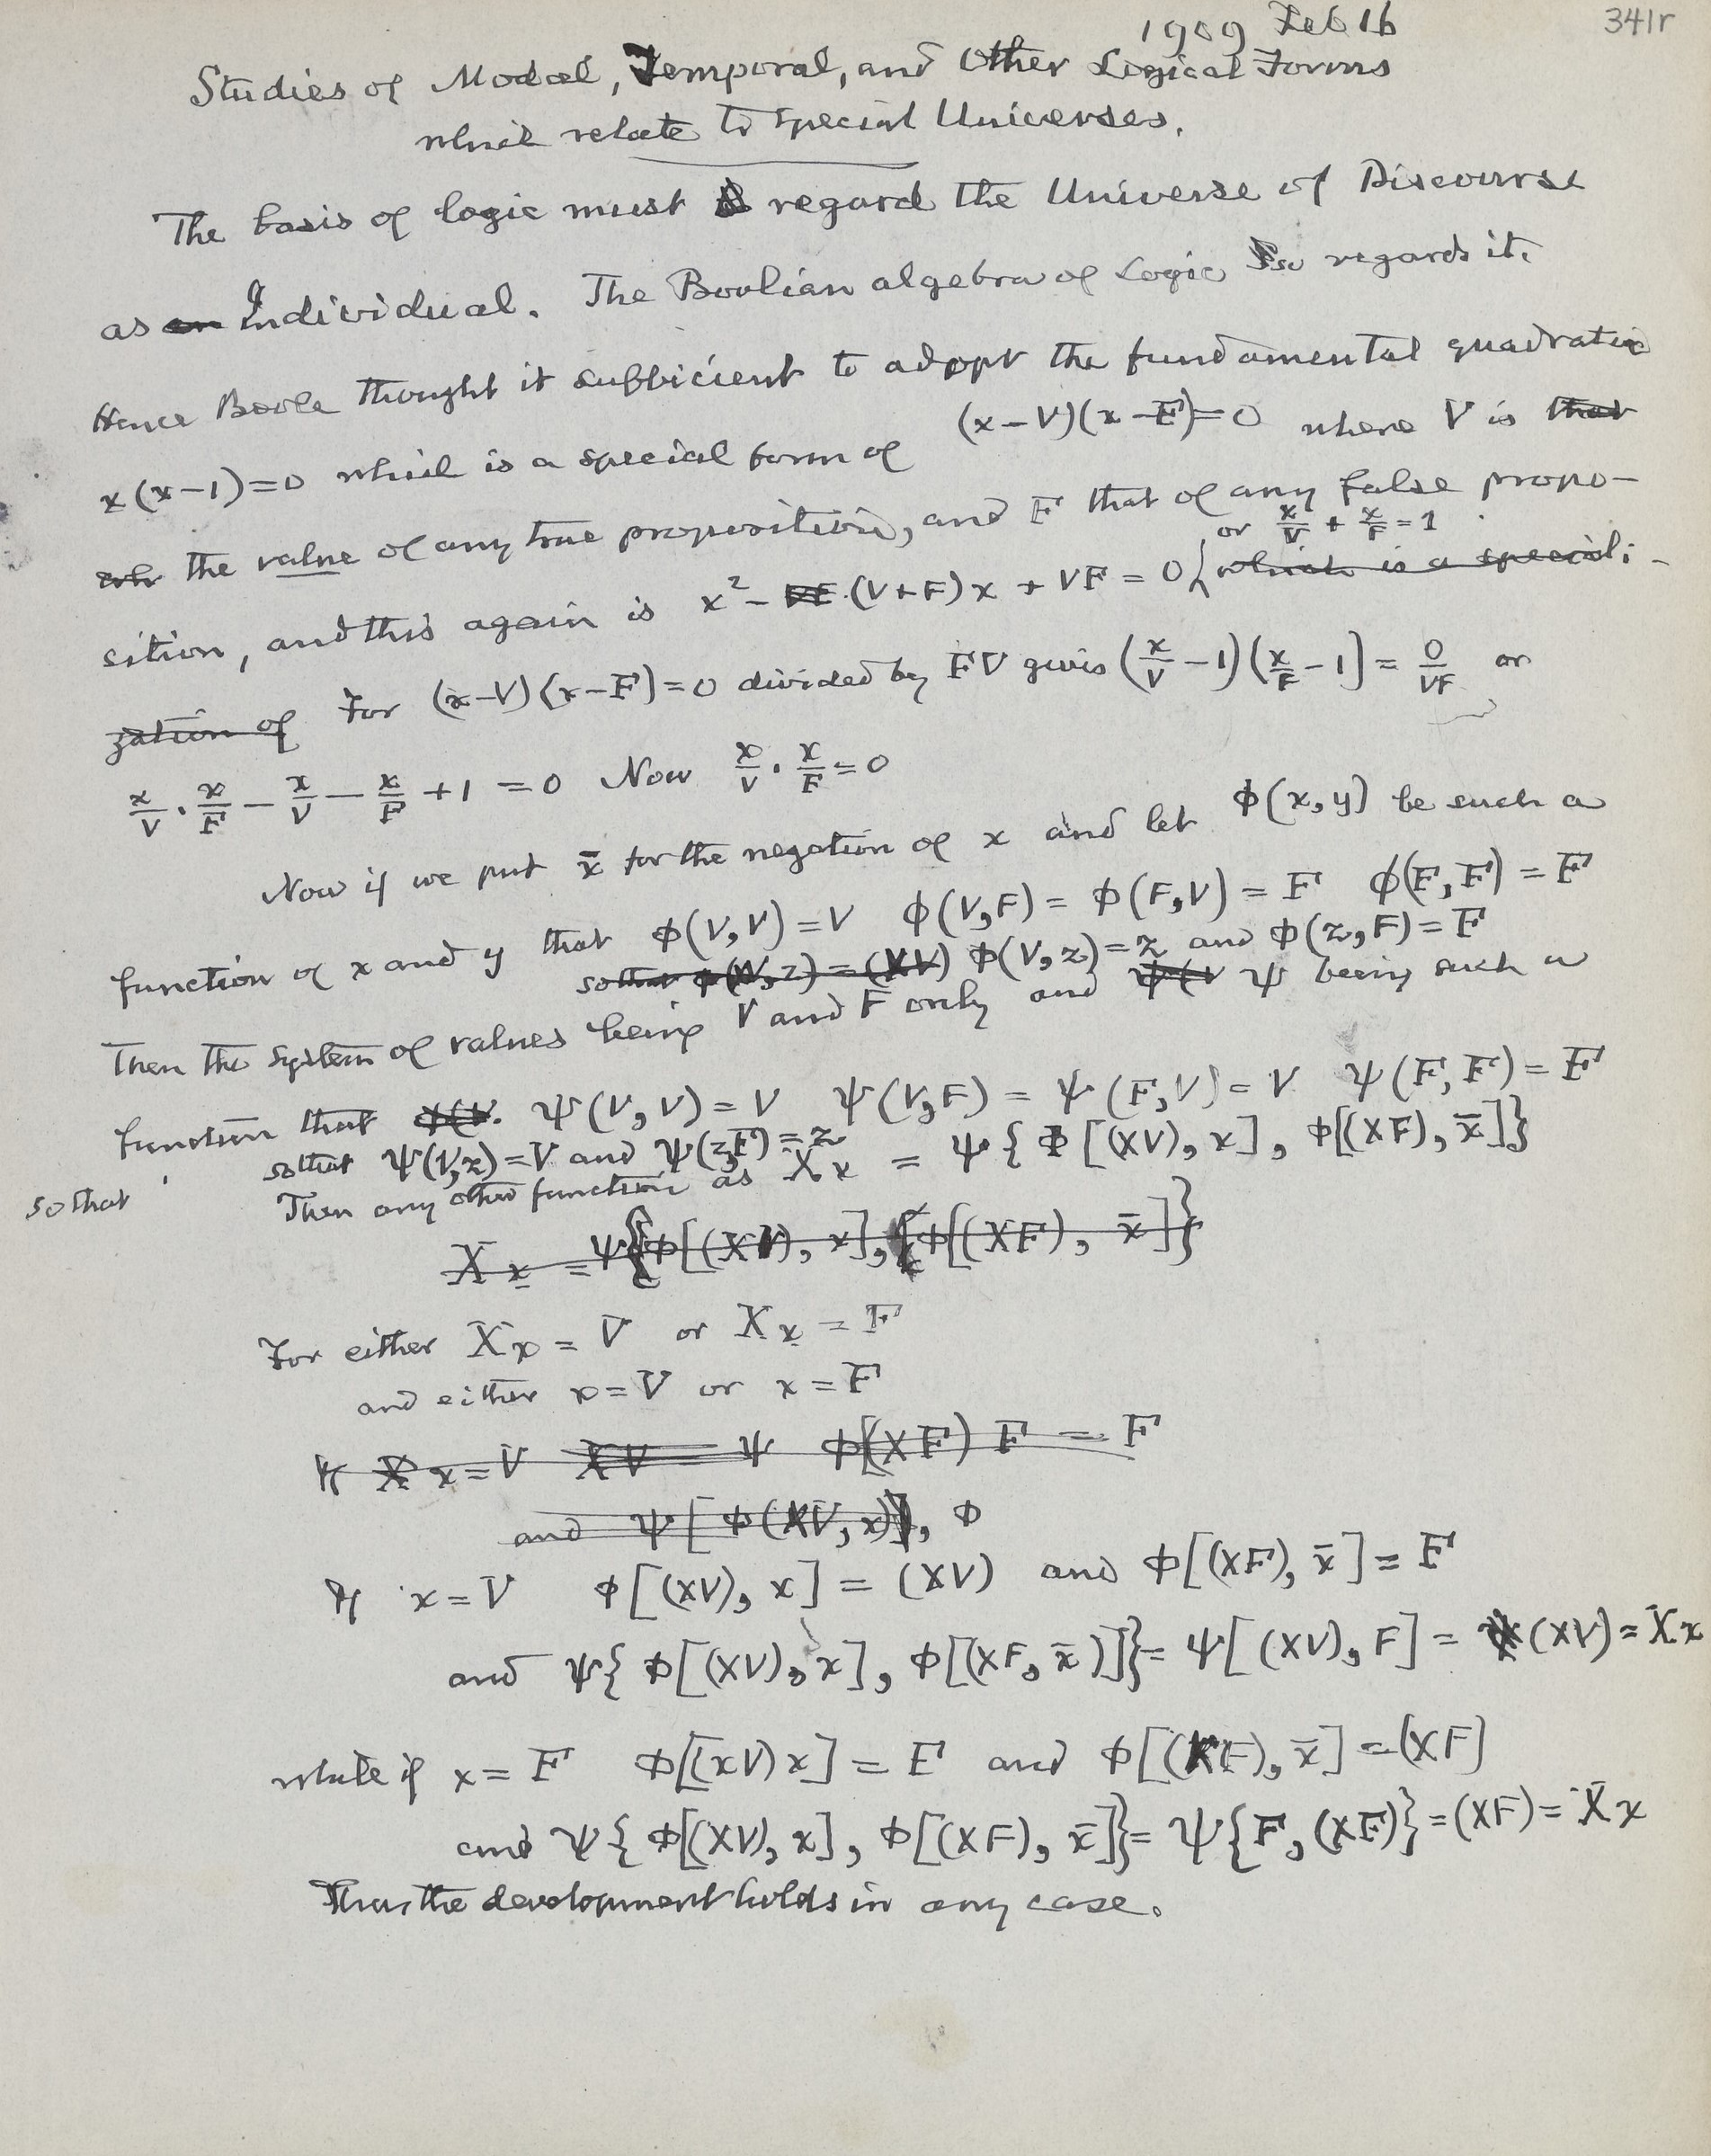
\includegraphics[width=\textwidth]{images/seq639.jpg}
    \caption{seq. 639 R.}
    \label{fig:639r}
\end{figure}

The next page up for discussion is the \textit{recto} that lies between the first two \textit{versos} that Fisch and Turquette discuss in their article. It is one of the few pages in Peirce's notebook that lends itself to a straightforward transcription. The page is dated February 16th, 1909 and its title reads as follows:

\begin{center}
\displayquote{``Studies of Modal, Temporal, and Other Logical Forms which relate to special Universes.''}
\end{center}

Here Peirce gives some further indication of the subject matter he is trying to capture, which appears to have something to do with temporal and modal propositions. It is unclear what the ``Other Logical Forms'' being referred to are, but one possibility is second order propositions since he had distinguished between first order and second order logic since at least 1885. But what does he mean by special universes? Elsewhere when Peirce speaks of special universes, it is in connection with his metaphysical categories and the ``modes of being'' discussed in section 3 of this chapter. In the same notebook, on August 28th in 1908, Peirce writes of ``the co-reality of three universes[:] 1st of ideas, 2nd of occurrences (existent things and actual events), [and] 3rd of powers to bring two substances $[\!\![$?$]\!\!]$, (and I will call powers of this sort Reasons), [which] must, accordingly, be supposed capable of rational explanation''(MS 339, \href{https://iiif.lib.harvard.edu/manifests/view/drs:15255301$550i}{seq.550}).\footnote{Fisch and Turquette draw attention to this passage as well.} This is most likely what Peirce was referring to when he writes ``special universes.'' Just as his `modes of being' are interpreted modally, so are his special universes. Peirce goes on to frame these special universes within his greater theory of ``hypothetical cosmology'' (\href{https://iiif.lib.harvard.edu/manifests/view/drs:15255301$555i}{seq. 555}).

The pages where Peirce elaborates this notion appears to be an outline of some kind. Based on the elaborations on the subsequent pages, we can infer that the `possibles' he is talking about do not necessarily only have the mode of being of possibility because they are unknown. They are not merely epistemically indeterminate. He calls them ``Real possibles.'' The `Reasons' he refers to are ``Real general Reasons, which do not merely exist in any mind of minds knowing that the denial of them are in no actual occurrence true.'' This is connected to something like what we might call `laws of nature.' For both of these concepts, Peirce is adamant in this passage that whatever they are is not `merely' epistemological. Their status as ``Possibles'' or ``Reasons'' is not based on our knowing whether they could pertain or our knowing that they could not not pertain. Peirce was an ardent defender of realism as opposed to nominalism, so this is likely the reason for this qualification.

The first paragraph on the page reads:
\begin{quotation}
\noindent``The basis of logic must regard the Universe of Discourse as individual. The Boolian algebra of Logic so regards it. Hence Boole thought it sufficient to adopt the fundamental quadratic $x(x-1)=0$ which is a special form of $(x-V)(x-F)=0$ where $V$ is the value of any true proposition, and $F$ that of any false proposition, and this again is $x^{2}-(V+F)x+VF=0$ (or $\frac{x}{V} +\frac{x}{F}=1$). For $(x-V)(x-F)=0$ divided by $FV$ gives $(\frac{x}{V} -1)(\frac{x}{F} -2)=\frac{0}{VF}$ or $\frac{x}{V} \cdot \frac{x}{F}-\frac{x}{V}-\frac{x}{F}+1=0$. Now $\frac{x}{V} \cdot \frac{x}{F}=0$''
\end{quotation}
\noindent The fundamental quadratic that Peirce refers too can be read as saying `it is false that some $x$ is not $x$' (as Boole used formulae of the form $x(1-y)$ to express `some $x$ is not $y$').\footnote{This is essentially a version of the Law of Identity.} The formula he says this is a special version of is a kind of ``elective expression,'' which in this case is simply the principle of non-contradiction (PC). Throughout this page he appears to be trying to extend this notion rather than refute it. Although, it is difficult to say what he was up to here because division does not seem to be part of Boole's notation, so it is unclear what he means when he writes expressions like $\frac{x}{V}$. One interpretation of the work on this page is that Peirce is attempting to modify an essentially Boolean system so that it can represent propositions involving the `special universes' he mentions in the title. If I am correct about the connection between these and the universes he described a few months prior, then he may have been trying to extend the scope of logic to propositions about possibilities and ``Reasons'', which might be understood as something like necessities.

Next $\Phi$ and $\Psi$ make an appearance again:
\begin{quotation}
``Now if we put $\bar{\lnot}x$ for the negation of $x$ and let $\Phi(x,y)$ be such a function that $\Phi(V,V)=V$, $\Phi(V,F)=\Phi(F,V)=F$, $\Phi(F,F)=F$. Then the system of values being $V$ and $F$ only and $\Psi$ being such a function that $\Psi(V, V)= V$ , $\Psi(V, F)=\Psi(F, V)=V$ , $\Psi(F, F)=F$

So that $\Psi(V, z)=V$ and $\Psi(x, F)= z$''
\end{quotation}
\noindent It may be worth noting that these formulations are inconsistent with the matrices written on the back of this page. Here it seems $\Phi$ and $\Psi$ have switched roles and now $\Phi$ is playing the role of conjunction and vice versa. In other regards they are consistent with the treatment of conjunction and disjunction in classical logic. He goes on to say:
\begin{quotation}
``Then any other function as $Xx=\Psi\{\Phi[(XV), x], \Phi[(XF),\bar{x}]\}$

For either $Xx=V$ or $Xx=F$

and either $x=V$ or $x=F$.''
\end{quotation}

\noindent This portion of the text helps to make sense of some of what appears on the first page Fisch and Turquette concern themselves with (seq. 639, \ref{fig:639r}). The portion of the page labelled (2) now appears to be making use of or working out a one place operator, $X$. So, when $XV$ appears within formulae in (4) and (5) of that same page, what is really meant is $X$ of $V$, $F$, or $x$. Here Peirce has given us a definition of that operator, however, the definition is clearly circular. This is likely no accident, and may have a connection with the third truth value, $L$, that appears on the other pages. Interpreting $\Phi$ as a kind of conjunction, and $\Psi$ as a kind of disjunction, we can see that $Xx$ will be reduced to either $XV$ or $XF$ depending on whether $x$ is true or not. If $x$ is true, then the right disjunct will be false, since $\bar{\lnot}x$ will be false, and the truth of the right disjunct will depend on the value assigned to $XV$. Likewise, if $x$ is false, then the value of $Xx$ will be whatever the value of $XF$ turns out to be. But of course we do not know what $XV$ or $XF$ will be because $X$ is used in its own definition. Peirce goes on to spell this out himself:
\begin{quotation}
``If $x=V$, $\Phi[(XV), x]=(XV)$ and $\Phi[(XF), \bar{x}]=F$

and $\Psi\{\Phi[(XV), x],\Phi[(XF), \bar{x}]\}=\Psi[(XV), F]= (XV)=Xx$

While if $x=F$, $\Phi[(XV), x]=F$ and $\Phi[(XF), \bar{x}]=(XF)$

and $\Psi\{\Phi[(XV), x],\Phi[(XF), \bar{x}]\}=\Psi\{(F, (XF)\}= (XV)=Xx$.''
\end{quotation}
The circular nature of the definition of $X$ might have some connection with the philosophical worries that led Peirce to begin these experiments in the first place. Perhaps it was introduced to represent portions of propositions whose truth value is either unknown or is fundamentally indeterminate. Peirce concludes this page stating ``Thus the development holds in any case.'' It is unclear what development Peirce is talking about but it likely has something to do with $X$. When he says it holds in any case, he may mean that it holds whether $x$ is true or false as in classical logic since maintaining this consistency seems to have been a priority.
%According to Richard he's showing that  X holds when the values are only T and F, and on the next page he is checking to see if it works for 3 values.

\section{seq. 641 R.}

\begin{figure}
    \centering
    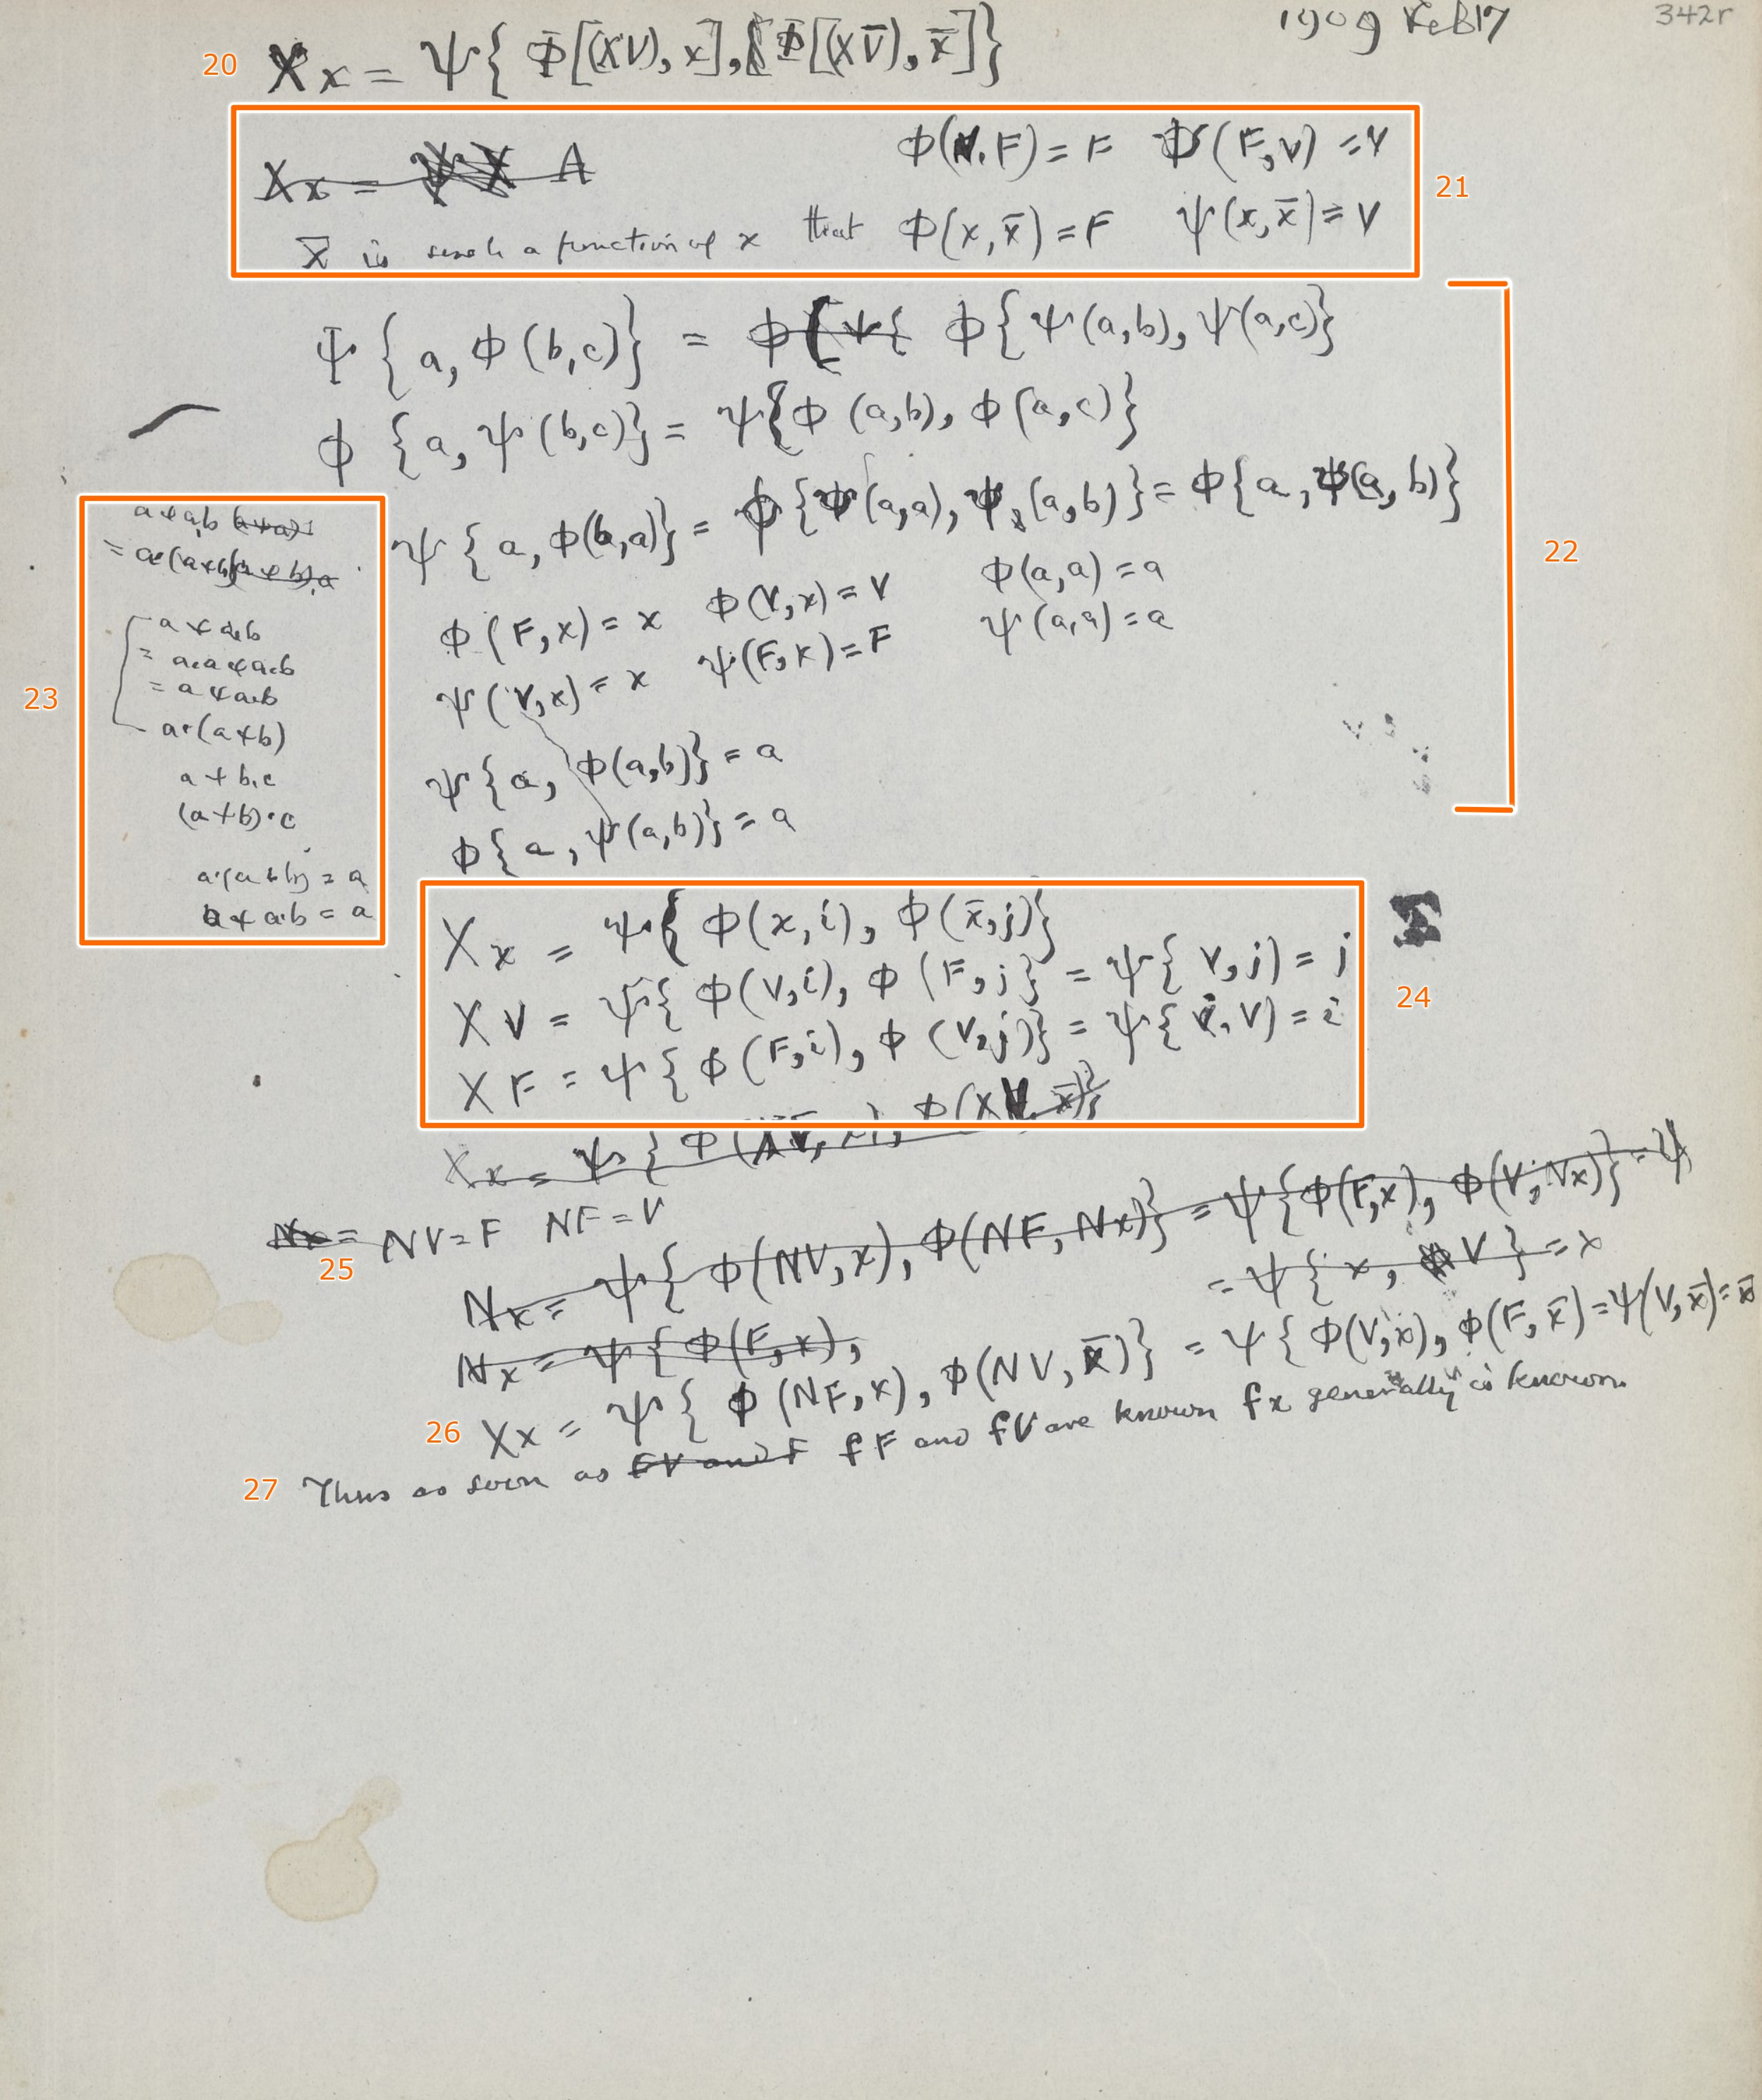
\includegraphics[width=\textwidth]{images/seq641.jpeg}
    \caption{seq. 641 R.}
    \label{fig:641}
\end{figure}

The final page in this group is a \textit{recto} following the second page Fisch and Turquette take up. It is dated February 17th, 1909.

The page begins (20) by recapitulating the definition for $X$. The only difference between the definition here and that of the previously discussed page is that instead of $F$ Peirce writes $V$ with a line above to symbolize its negation: ``$Xx=\Psi\{\Phi[(XV), x], \Phi[(X\bar{V}),\bar{x}]\}$''. This doesn't seem to amount to a significant change.

In (22) he restates some features of $\Phi$ and $\Psi$ as well as the negation operator, $\bar{\lnot}x$ (which is presumably the three-valued version). It reads ``$\Phi(V,F)=F$, $\Psi(F,V)=V$'' and then states that ``$\bar{\lnot}x$ is such a function that $\Phi(x,\bar{x})=F$ [and] $\Psi(x, \bar{x})=V$.'' So again, $\Phi$ and $\Psi$ are working like regular conjunction and disjunction. It also seems as though he is trying to show that the laws of non-contradiction and excluded middle still hold with regard to $\bar{\lnot}x$. 

Immediately below (22), he gives some basic equivalences between $\Phi$ and $\Psi$ formulae before giving formulations that contradict what is written of $\Phi$ and $\Psi$ in (21) and seq. 639. It seems that either here or while scribbling on the \textit{verso} facing this page Peirce had decided to switch the roles of $\Phi$ and $\Psi$. $\Phi$ is now a kind of disjunction and $\Psi$ now a kind of disjunction. There is no apparent reason for doing this, so it likely came down to personal preference.

To the left (23), there appears to be some scratch work that contains formulae misshapen $+$ signs, which could be $\Psi$s but are more likely regular two valued disjunctions. They appear alongside $\cdot$s, which are normally two valued conjunctions in Peirce's notation. The connectives are combining arbitrary atomic sentences, but it is unclear what the overall significance of this is.

In (24), we find more formulations with $X$. He writes:
\begin{quotation}
``$\Psi\{\Phi(x, i),\Phi(\bar{x}, j)\}$

$\Psi\{\Phi(V, i),\Phi(F, j)\}=\Psi(V,j)=j$

$\Psi\{\Phi(F, i),\Phi(V, j)\}=\Psi(i,V)=i$''
\end{quotation}
\noindent One difference between these formulations and his previous characterization of $X$ is that $\Psi$ and $\Phi$ roles have switched, which is consistent with (22), yet $\Psi$ is still the primary operator in the definitions. Another difference is that the circularity of the previous definition has been dropped. $X$ no longer features in its own definition. The final difference is that $i$ and $j$ have been added to the mix aside from $x$, $V$, and $F$. He may have had specific interpretations in mind for these, but the only other place they show up in these pages is in \href{https://iiif.lib.harvard.edu/manifests/view/drs:15255301$637i}{seq. 637}, where they are winners and losers. It is doubtful that this is what they mean here though.

The next line (25) introduces something new. Here Peirce has written ``$NF=F$ [and] $NF=V$.'' He tells us very little about this new operator but it may be of a similar kind to $X$. One possibility is that these were intended to be kinds of modal operators, as he seems to have been concerned with modality on previous pages. It is unclear whether either of them are intended to be truth-functional. Nevertheless, $N$ appears in connection with $X$ in the next line (26): ``$Xx=\Psi\{\Phi(NF, x), \Phi(NV, \bar{x})\}=\Psi\{\Phi(V,x),\Phi(F,\bar{x}\}=\Psi(V,\bar{x})=\bar{x} $.'' This formula is basically the same as the definition for $X$ on the previously discussed page except the $X$s on the right of the identity symbol are replaced with $N$s. But since we know that $NF=F$ and $NF=V$, the value of the formula is able to be reduced to the value of $\bar{\lnot}x$. 

The most interesting part of the page is likely the last line(27). In it Peirce states ``Thus as as soon as $fF$ and $fV$ are known $fx$ is generally known.'' The $f$ here seems most likely to be an arbitrary place holder for unary functions like $X$ and $N$. It is unclear how best to interpret this. It is possible that Peirce may simply be claiming that if you know what a function on \textit{Verum} and \textit{Falsum} give you, then figuring out what that function gives on any arbitrary proposition is a trivial matter.
